\chapter{Dump}
\label{chap:sm}


\section{Semileptonic Decays, specifically $B_s \to D_s l \nu$}
\label{sec:semileptonic}

The key motivations for studying decays like the $B_s \to D_s l\nu$ are:
\begin{itemize}
	\item
	Determination of CKM matrix elements. Specifically, by combining the theoretical prediction and an observed brancing fraction of $B_s \to D_s l\nu$, $|V_{cb}|$ can be extracted.
	\item
	Precision tests of the standard model. There are currently a number of tensons between experiment and the standard model predictions of $B$ decays, some closely related to $B_s \to D_s l\nu$ \cite{Na:2015kha}.
\end{itemize}
We will first discuss the general ideas in computing semileptonic decays.
%-------------------------------------------------------------------------------------

\subsection{Semileptonic Decays}
\label{sec:cp}

\begin{wrapfigure}{R}{0.55\textwidth}
  \begin{center}
  \vspace{-25pt}
    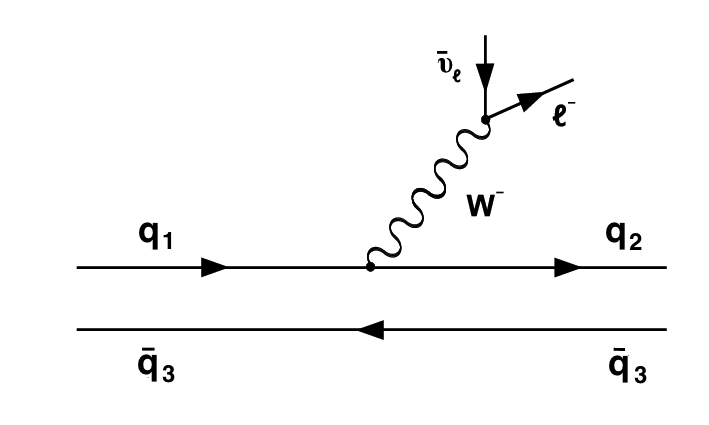
\includegraphics[width=
   0.5\textwidth]{images/semileptonic.png}
     \vspace{-25pt}
  \end{center}
  \caption{Semileptonic decay at tree level}
  \vspace{+10pt}
  \label{fig:semileptonic}
\end{wrapfigure}

Semileptonic decays are useful for studying the sector of the standard model (SM) which couples quarks to the weak force \cite{Richman:1995wm}:
\begin{align}
 \mathscr{L}_{W} & = {g\over\sqrt{2}} \left[ \quad V_{ij} J_{ij}^{\mu} W_{\mu}^+ + V^{\dagger}_{ij} J_{ij}^{\mu \dagger} W_{\mu}^- \quad \right]
  \label{eq:weakL}
\end{align}
$J_{\mu}^{ij} = \bar{u}_i \gamma_{\mu} {1\over2}(1-\gamma_5) d_j$ are the weak currents,
$\underline{u} = ( u, c, t )$ and $\underline{d} = ( d, s, b )$ are the quark fields, $g$ is the weak coupling constant, $W^{\pm}$ are the charged weak bosons, and $V$ is the (unitary)
Cabibbo-Kobayashi-Maskawa (CKM) matrix. $V_{ij}$ can be thought of as a matrix of couplings which dictate the probability
of mixing between two quark flavours, for example the amplitude of a $b$ decaying to a $u$ (and emitting a $W$) is proportional to $V_{13} \equiv V_{ub}$.
\\ \\
A semileptonic decay is any $hardon\to hadron+leptons$ process. Fig. \ref{fig:semileptonic} shows the tree level (in weak coupling) contribution to a semileptonic decay. We denote a meson with valence quark content $q$ and $q'$ as $M_{qq'}$. The $M_{q_1\bar{q}_3} \to M_{q_2\bar{q}_3} l \bar{\nu}_l$ decay ($l$ is some charged lepton and $\bar{\nu}_l$ is it's neutrino) is proportional to $V_{q_1q_2}$ at tree level.
\\ \\
This is given by
\begin{align}
  \mathcal{M} = \left({ig\over\sqrt{2}}\right)^2 V_{q_1q_2} \langle M_{q_2\bar{q}_3}, l\bar{\nu} | J_{\alpha}^{q_1\bar{q}_2} D^{\alpha\beta}_W(p^2) J^{l\bar{\nu}}_{\beta} | M_{q_2\bar{q}_3} \rangle
\end{align}
$J^{l\bar{\nu}}$ is the analog of the quark currents $J^{q_1\bar{q}_2}$, since the $W$ couples in the same way to leptons (with $V$ replaced by a unit matrix).
If the external momenta of the process $p^2$ are much smaller than the $W$ mass, one can remove the $W$ propagator from the tree level amplitude \cite{Borasoy:2007yi};
\begin{align}
 \left({ig\over\sqrt{2}}\right)^2 D^{\mu\nu}_W(p^2) = \left({ig\over\sqrt{2}}\right)^2 \left( -ig^{\mu\nu} \over p^2 - M_W^2 \right)
  & = \underbrace{ {i\over M_W^2} \left( ig \over \sqrt{2} \right)^2  }_{\equiv -2\sqrt{2}G_F} g^{\mu\nu} + \mathcal{O}\left({p^2\over M_W^4}\right)
\end{align}
Then $\mathcal{M}$ can be factorised;
\begin{align}
  \nonumber
  \mathcal{M} & \simeq -2\sqrt{2} G_F V_{q_1q_2} \langle M_{q_1\bar{q}_3}, l\bar{\nu} | J_{\mu}^{q_1\bar{q}_2} J^{l\bar{\nu} \mu} | M_{q_2\bar{q}_3} \rangle \\
  \nonumber
  & = -2\sqrt{2} G_F V_{q_1q_2} \langle l\bar{\nu} | J^{l\bar{\nu} \mu} | 0 \rangle \langle M_{q_1\bar{q_3}} | J_{\mu}^{q_1\bar{q}_2} | M_{q_2\bar{q}_2} \rangle \\
  & \equiv -2\sqrt{2} V_{q_1q_2} G_F L^{\mu} H_{\mu}.
  \label{eq:LH}
\end{align}
$L_{\mu}$ can be computed in perturbation theory. The hadronic matrix element $H_{\mu}$ however, due to the non-perturbative nature of QCD at low energies,
cannot be computed analytically. It is quantities such as $H_{\mu}$ that we wish to calculate in lattice QCD.

\subsection{CKM Extraction}

Speaking heuristically, if one can calculate the quantity $G_F L^{\mu} H_{\mu}$ from theory, and measures the amplitude of the process $\mathcal{M}$, they could then rearrange equation \eqref{eq:LH} to deduce $V_{q_1q_2}$. Speaking more practically, the relevant equation is, for example, for the $B_s \to D_s l\nu$ decay \cite{Na:2015kha}:
\begin{align}
	{d\Gamma \over dq^2} =& \eta_{\text{EW}} {G^2_F |V_{cb}|^2 \over 24\pi^3 M_{B_s}^2} \left( 1 - {m_l^2\over q^2}\right)^2 |\underline{p}| \\
	&\times \left[ \left(1+{m_l^2\over 2q^2}\right) M_{B_s}^2 |\underline{p}| f^2_+(q^2) + {3m_l^2\over 8q^2}(M_{B_s}^2 - M_{D_s}^2)^2 f_0^2(q^2)\right]
\end{align}
where $m_l$ is the mass of the charged lepton, $\eta_{\text{EW}}$ is an electroweak correction factor, $q^2$ is the momentum transfer, ${d\Gamma/dq^2}$ is the branching fraction, and $f_{0,+}(q^2)$ are the form factors associated with the decay, to be defined in \ref{sec:formfactors}. Given experimental data for ${d\Gamma/dq^2}$ and theoretical data for $f_{0,+}(q^2)$, one can deduce $|V_{cb}|$.
\\ \\
What is the value of determining CKM elements? Firstly, uncertainty in CKM elements are the dominant error in many standard model predictions. $V$ elements can also test the standard model. $V$ is unitary by definition. However, if there were more than 3 generations of quark, requiring $V$ to be 4x4 or larger, the 3x3 submatrix which couples the 3 known generations
would not itself be unitary in general (\cite{Schwartz:2013pla} ch. 29). Therefore, if one can deduce the elements of the 3x3 $V$ to high enough precision to show it is not unitary, this would be indirect evidence for new physics. 
\\ \\
Unitarity imposes a constraint on each row of $V$. The current status of the unitarity of $V$ can be read off from below (each quantity should be zero for unitarity to hold)\cite{Aoki:2016frl}:
\begin{align}
	\nonumber
	&|V_{ud}|^2 + |V_{us}|^2 + |V_{ub}|^2 - 1 = -0.020(9) \\ 
	&|V_{cd}|^2 + |V_{cs}|^2 + |V_{cb}|^2 - 1 = 0.06(3)
\end{align}
both of the above relations display a $\sim2\sigma$ deviation from unitarity. More precise values of these parameters are needed to discover if CKM is infact non-unitary.
\\ \\
Now we consider $|V_{cb}|$ specifically. $|V_{cb}|$ is the dominant uncertainty in many standard model predictions of rare decays, such as $B_s \to \mu^+\mu^-$,$K\to\pi\nu\bar{\nu}$, and the CP violation parameter $\epsilon_K$ \cite{Na:2015kha}. The FLAG working group quotes their average $|V_{cb}|$ to currently be \cite{Aoki:2016frl}:
\begin{align}
	|V_{cb}| = 0.04085(95)
\end{align}
However, the water is slightly muddied by the presence of tensions between different determinations of $|V_{cb}|$, namely between that deduced from studying $B\to D^*l\nu$, and an inclusive analysis of $B\to X_c l\nu$ where $X_c$ is any meson containing a $c$ quark \cite{Na:2015kha}:
\begin{align}
	|V_{cb}|_{\text{inclusive}} = 0.04221(78) \text{ , } |V_{cb}|^{B\to D^* l\nu} = 0.03904(49)_{\text{expt.}}(53)_{\text{QCD}}(19)_{\text{QED}}
\end{align}
A recent review of $|V_{cb}|$ determinations from the lattice is given in \cite{Wingate:2017unz}. This issue would benefit from a $|V_{cb}|$ determination from annother channel, like $B_s\to D_s l\nu$, to flesh out the landscape of $|V_{cb}|$ values and pinpoint the source of the tension, if there is any.

\subsection{Lepton Flavour Violation}
\label{sec:anomalies}

There are a number of tensions currently between theory and experiment in $B$ decays, who's true nature can be eludicated by our $B_s\to D_s l\nu$ study, and eventual $B\to Dl\nu$ study.
\\ \\
Define the ratios
\begin{align}
	R(X) = {\mathcal{B}(B\to X \tau \nu_{\tau}) \over \mathcal{B}(B\to X l \nu_l)}
\end{align}
where $l=e$ or $\mu$. These can be computed either purely from a lattice calculation, or purely from experimental data, independantly of the associated CKM element. It therefore can be used for comparison between experiment and the standard model. $R(D^*)$ contains a $~2.1\sigma$ discrepancy \cite{Aaij:2015yra}:
\begin{align}
	R(D^*)|_{\text{SM}} = 0.252(3) \text{ , } R(D^*)|_{\text{LHCb}} = 0.336(27)_{sys}(30)_{stat}
\end{align}
The issue is similarly present for $R(D)$ \cite{Monahan:2017uby}:
\begin{align}
	R(D)|_{\text{SM}} = 0.299(7) \text{ , } R(D)|_{\text{exp}} = 0.391(28)_{sys}(41)_{stat}
\end{align}
where in this case $R(D)|_{\text{expt}}$ is a world average of experimental values. Our eventual study of $B\to Dl\nu$ will produce a new standard model determination of $R(D)$, helping shed light on the issue.
\\ \\
\begin{figure}
  \begin{center}
    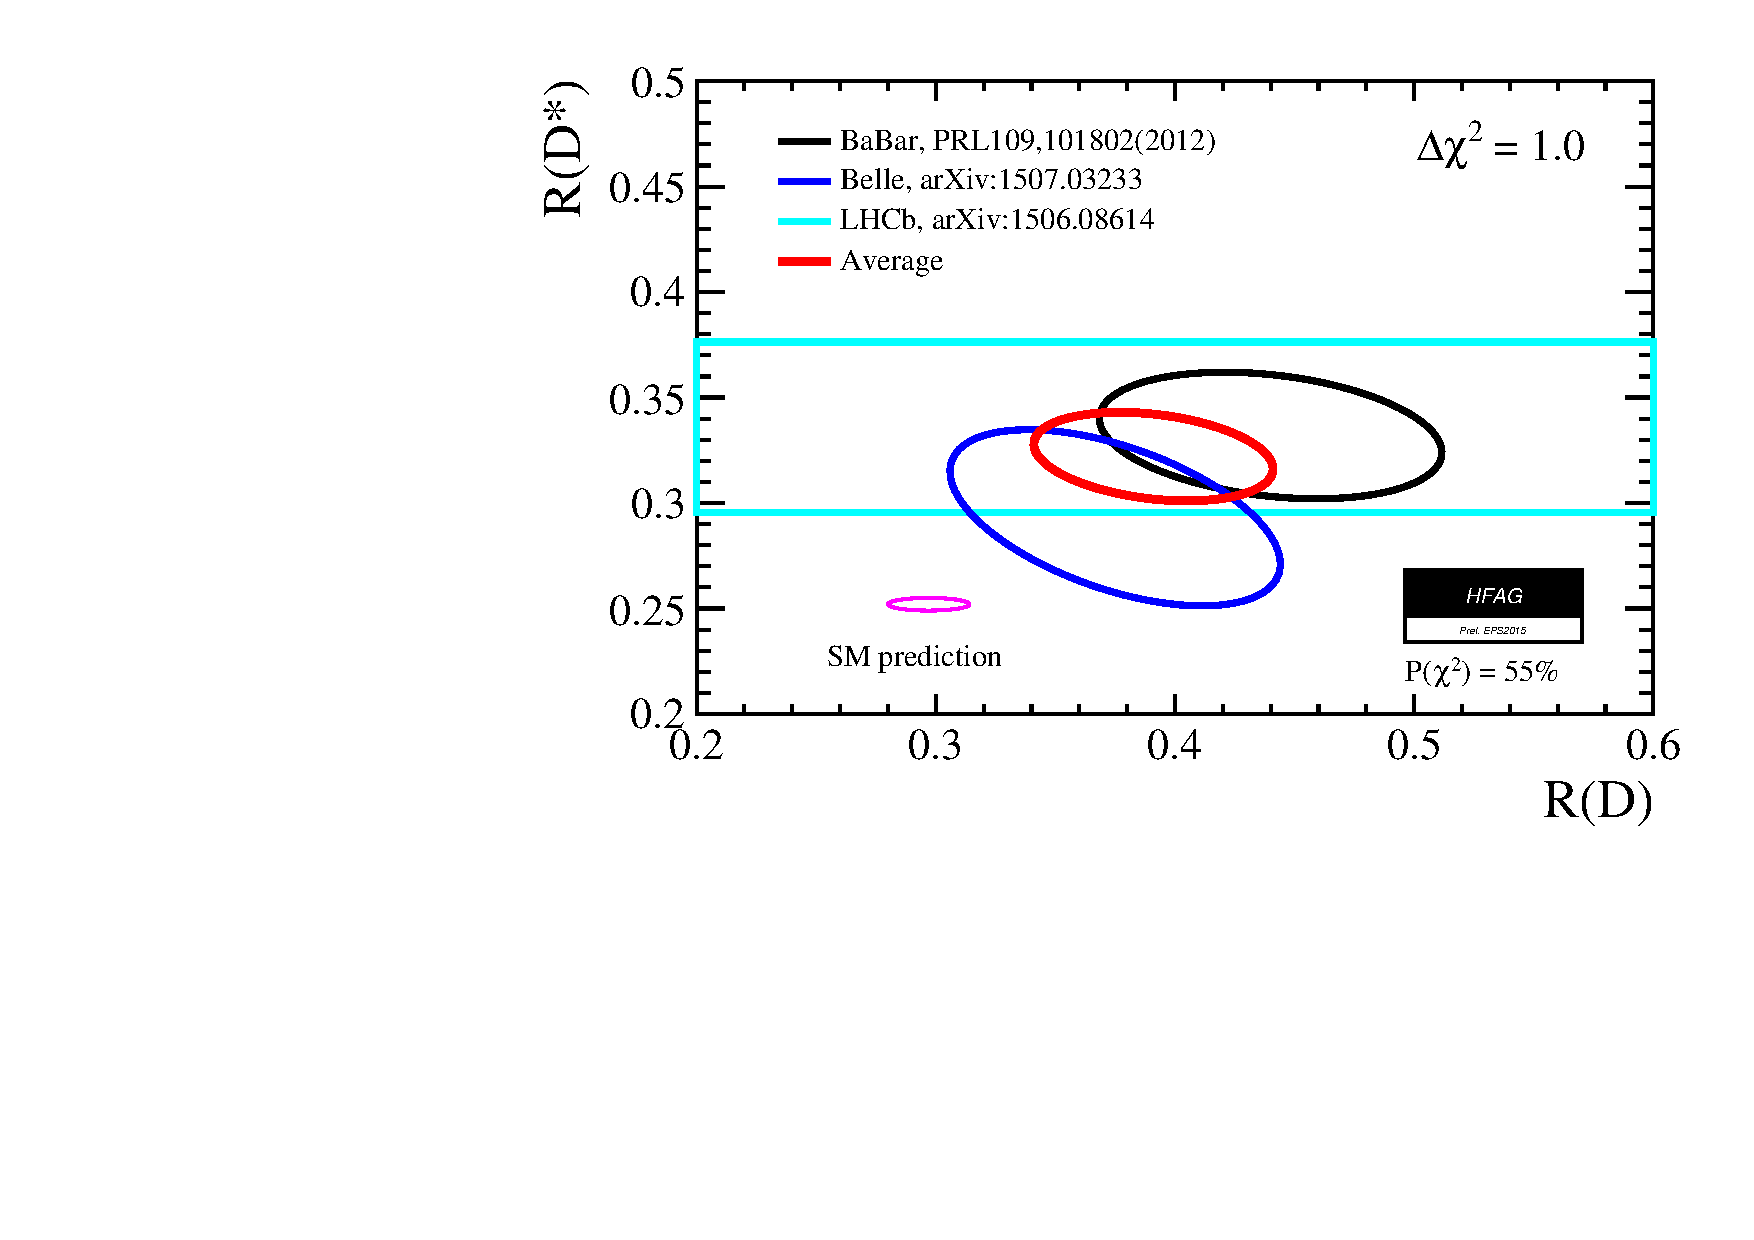
\includegraphics[width=
   0.8\textwidth]{images/rdrds_eps15.pdf}
  \end{center}
  \caption{$R(D)/R(D^*)$ determinations from standard model and experiment \cite{HFAG}}
  \label{fig:semileptonic}
\end{figure}
%A natural question to ask is: is there an analagous tension in related channels, like $B_s\to D_s l\nu$? There is not yet any experimental data for this decay, but the current best standard model determination is given by ${\mathcal{B}(B_s\to D_s \tau \nu_{\tau}) / \mathcal{B}(B_s\to D_s l \nu_l)} |_{\text{SM}} = 0.314(6)$.
\\ \\
Besides these, there are also tensions in the quantitites \cite{Altmannshofer:2017yso}:
\begin{align}
	R'(K^{(*)}) = {\mathcal{B}( B\to K^{(*)}\mu^+\mu^-)\over \mathcal{B}( B\to K^{(*)} e^+e^-)}
\end{align}
All of the above anomalies are suggestive of lepton flavour violating effects. Various BSM models have been suggested; hot topics include Leptoquarks, $Z'$ models, and partial compositeness \cite{Altmannshofer:2017yso}.

\subsection{Kinematics and Form Factors}
\label{sec:formfactors}

We now turn to some more technical details about semileptonic decays.
\\ \\
We will refer to the 4-momenta and mass of the initial and final states as $p_{1,2},M_{1,2}$ respectively, and define the 4-momentum taken away by the $W^{\pm}$ boson as $q \equiv p_2 - p_1$. We work in the rest frame of the initial meson, in which
\begin{align}
	q^2 = M_1^2 + M_2^2 - 2M_1 E_2.
\end{align}
There is a physically allowed range of values for an on-shell $q^2$. The minimum is when all of the 3-momentum of the initial state is taken by the final meson, $q_{\text{min}} ^2 = 0$. $q^2$ is maximised when all of the 3-momentum is taken by the boson, $\underline{p}_2^2 = 0 \rightarrow E_2 = \sqrt{M_2^2 + \underline{p}_2^2 } = M_2 \rightarrow q_{\text{max}}^2 = M_1^2 - M_2^2 - 2M_1M_2 = ( M_2 - M_1 )^2$. So
\begin{align}
	0 \leq q^2 \leq ( M_2 - M_1 )^2
\end{align}
This also creates an allowed range for the final meson 3-momentum:
\begin{align}
	0 < \underline{p}_{2}^2 < \left( M_1^2 + M_2^2 \over 2M_1 \right)^2 - M_2^2
\end{align}
\\ \\
Hadronic matrix elements like $H_{\mu}$ from sec. \ref{sec:cp} can be parameterised in terms of form factors. The current operator between between the states is a conserved current, so then the matrix element must be proportional to only conserved quantities, namely, elements of the stress-energy tensor. Lorentz invariance requires indices on either side of such a relation match, so a matrix element with a single Lorentz index can only be proportional to 4-momenta.
\\ \\
Let us consider the case where the two states in the matrix element are pseudoscalar mesons (as in $B_s\to D_s l\nu$), with an insertion of a left-handed current (i.e. the coupling to the $W^{\pm}$ in \eqref{eq:weakL}), $J_{\mu}^{ij} = \bar{u}_i \gamma_{\mu} {1\over2}(1-\gamma_5) d_j$. This can be written as $J^{ij}_{\mu} = V^{ij}_{\mu} - A^{ij}_{\mu}$, these are the vector and axial vector currents. 
\\ \\
The axial vector evaluated between two pseudoscalar states must vanish because the combination is not parity invariant thus does not contribute in pure QCD, leaving just the vector current. The most common parameterisation is:
\begin{align}
\label{eq:formfactors}
\langle P_2 (p_2) | V^{\mu} | P_1 (p_1) \rangle  &= f_{+} (q^2) \left[ p_1^{\mu} + p_2^{\mu} - {M_1^2 - M_2^2 \over q^2} q^{\mu} \right] + f_0(q^2) {M_1^2 - M_2^2 \over q^2 } q^{\mu}
\end{align}
Where $|P_i(p_i)\rangle$ is a pseudoscalar meson state with momentum $p_i$.

%-------------------------------------------------------------------------------------

\section{Lattice QCD}
\label{sec:lat}

\subsection{Discretization}

At low energies ($\sim$200MeV and below), QCD becomes non-perturbative, in other words, the coupling $\alpha_s$ becomes $\mathcal{O}(1)$, and an expansion in $\alpha_s$ (as in perturbation theory) will not be dominated by the leading orders \cite{Schwartz:2013pla}. We require an alternative.
\\ \\
The expectation value of an observable $\mathcal{O}$ in a Yang-Mills theory can be expressed as a Euclidean path integral \cite{Lepage:1998dt};
\begin{align}
 \langle \mathcal{O} \rangle = \int \mathcal{D}A\mathcal{D}\psi\mathcal{D}\bar{\psi} \mathcal{O} e^{-S[A,\psi,\bar{\psi}]},
\end{align}
where $A$ is a gauge field, $\psi$($\bar{\psi}$) is an (anti)fermion field, $S$ is the Euclideanised classical action, and $\mathcal{D}$ denotes integration over all configurations of a field. "Euclideanised" refers to a Wick rotation $t\to it$ in $S$. In the perturbative approach, we would expand $\exp(-\text{interacting part of }S )$ resulting in a power series in
the gauge coupling populated by Feynman diagrams.
\\ \\
The other option is to instead carry out the integral directly. This can only be done numerically.
 Since it's not numerically feasible to carry out an infinite number of integrals, one must approximate spacetime as a discrete 4 dimensional lattice with spacing "$a$" between lattice sites, finite spacial volume $L_x^3$ and finite temporal extent $L_t$. The functional integral becomes
\begin{align}
 \int \mathcal{D}A\mathcal{D}\psi\mathcal{D}\bar{\psi} = \prod_{n} \int dU(x_n) d\psi(x_n) d\bar{\psi}(x_n),
\end{align}
where $n$ is a 4-vector with integer components labelling the sites, and $x_n^{\mu} = an^{\mu}$.
This has a second benefit which is to naturally regularize the theory with a momentum cutoff $\Lambda \sim 1/a$ \cite{Lepage:1998dt}. The gauge field has been replaced with the gauge
``link'':
\begin{align}
U_{\mu}(x) \equiv \exp\left(igaA_{\mu}\left(x+{a\hat{\mu}\over2}\right)\right) \in SU(N_c),
\end{align}
$g$ is the gauge coupling, $\hat{\mu}$ is a unit vector in the $\mu$ direction. Parameterizing the gauge fields this way is motivated by the geometrical interpretation of Yang-Mills theories on discrete spacetime and the requirement of exact gauge symmetry \cite{Munster:2000ez}.

\subsection{Meson Correlation Functions}
\label{sec:correlators}

A typical quantity that is computed on the lattice is a meson correlation function, i.e. when $\mathcal{O} = \Phi(x)\Phi^{\dagger}(y)$ and $\Phi$ is a meson creation operator. This is a good working example for showing the steps in a lattice calculation. 
\\ \\
A creation operator for a meson in this context can be any operator containing the same quantum numbers as the meson one is trying to create. For example, the neutral $B$ meson is a pseudoscalar charged with a $d$ and $\bar{b}$ quark, so a suitable operator is $\Phi(x) = \bar{b}(x)\gamma_5 d(x)$. The path integral can then be written as 
\begin{align}
	C(x,y) = \int \mathcal{D}\psi \mathcal{D}\bar{\psi} \mathcal{D}U \left(\text{ } \bar{b}(x)\gamma_5 d(x) \bar{d}(y)\gamma_5 b(y) \text{ }\right) e^{-S_G[U]-\sum_{w,z} \bar{\psi}(w)M(w,z)[U]\psi(z)}
\end{align}
where we have now broken the action up into a gauge part $S_G[U]$, and a fermion part. $M(x,y)[U]$ is the Dirac operator, and can be seen as a matrix in lattice site, flavor, color and spin. $\psi$ is a vector of quark flavours.
\\ \\
The integral over fermions can be preformed analytically, since the fermion fields are Grassman valued. In our example, the result is \cite{Peskin:1995ev},
\begin{align}
	C(x,y) = \int \mathcal{D}U \text{ Tr}\left[\text{ } M^{-1}_b(y,x)[U] \gamma_5 M^{-1}_d(x,y)[U] \gamma_5 \text{ }\right] e^{-S_G[U]} \text{det}(M[U])
\end{align}
The quantinties $M^{-1}_f(x,y)[U]$ are propagators of a quark of flavour $f$ on a fixed gauge background $U$. The integration over gauge fields is generally carried out by an importance sampling method. A finite \textit{ensemble} of gauge configurations $\{U_i\}$ is generated by a Monte Carlo Markov chain (MCMC), where the probability of a gauge configuration $U_j$ being added to the ensemble is proportional to 
\begin{align}
	e^{-S_G[U_j]}\text{det}(M[U])
	\label{eq:MCweight}
\end{align}
See \cite{DeGrand:2006zz} ch. 7 for examples of such algorithms. In the case of our work, we use ensembles generated by the MILC collaboration \cite{Bazavov:2012xda}.
\\ \\
Once the ensemble is created, the path integral can be approximated by simply
\begin{align}
  C(x,y) \simeq {1\over N} \sum_i \text{ Tr}\left[\text{ } M^{-1}_b(y,x)[U_i] \gamma_5 M^{-1}_d(x,y)[U_i] \gamma_5 \text{ }\right]
  \label{eq:av_gauge}
\end{align}
where $N$ is the size of the ensemble. The calculation of the correlation function then is split into 3 steps:
\begin{enumerate}
	\item
	Generate an ensemble of Gauge configurations $\{ U_i \}$ by MCMC.
	\item
	Compute quark propagators $M^{-1}_f(x,y)[U]$ on each Gauge configuration. This requires inverting the matrix $M$ each time, this is typically done by conjugate gradient method.
	\item
	Construct trace as in \eqref{eq:av_gauge}, and average over the ensemble.
\end{enumerate}
We now turn to the issue of choosing lattice actions.

\subsection{Gauge Action}
\label{sec:gauge}

One must choose a discrete version of $S$ which becomes the original Yang-Mills action in the limit $a\to0$. There are many choices of $S$ which satisfy this. The simplest action with a continuum limit coinciding with an $SU(N_c)$ gauge theory is
\begin{align}
   S_G = \beta \sum_{x,\mu,\nu} \left[ N_c - \text{Tr}\left( U_{\mu}(x) U_{\nu}(x+a\hat{\mu}) U^{\dagger}_{\mu}(x+a\hat{\nu}) U^{\dagger}_{\nu}(x) \right)  \right].
\end{align}
The trace is over colour, and $\beta = 2(L_x/a)/g^2$. The product of gauge links $U_{\mu}(x) U_{\nu}(x+a\hat{\mu}) U^{\dagger}_{\mu}(x+a\hat{\nu})U^{\dagger}_{\nu}(x)$ is known as the elementary plaquette, and is the lattice analogue of the field strenght tensor $F_{\mu\nu}$.
In practice this action is appended with irrelevant operators which act to cancel discretisation effects in the results of calculations, these are known as Symmanzik improvements (\cite{DeGrand:2006zz} ch.10). 
For example, in the MILC ensembles, the Gauge action used is a generalization of the above, the Luscher-Weisz action \cite{Gattringer:2001ia}.

\subsection{Fermion Actions}

The interacting Dirac action is most naively discretised with
\begin{align}
 S_F &= \sum_{x,\mu} \bar{\psi}(x) \gamma_{\mu} \nabla_{\mu} \psi(x) + m\sum_x \bar{\psi}(x) \psi(x),
 \label{eq:naivefermions}
\end{align}
where $\nabla_{\mu}$ is the gauge covariant finite difference operator,
\begin{align}	
	\nabla_{\mu} \psi(x) = {1\over 2a} ( U_{\mu} (x) \psi(x+a\hat{\mu}) - U^{\dagger}_{\mu}(x-a\hat{\mu})\psi(x-a\hat{\mu}) ).
\label{eq:lat_derivative}
\end{align}
In appendix \ref{sec:doublingprob} we describe the doubling problem. This is the observation that the propagator for a fermion obeying \eqref{eq:naivefermions}, $M^{-1}(k)$ has the property
\begin{align}
	M^{-1}(k+{\pi\over a}\zeta) = \gamma_{5\mu} M^{-1}(k) \gamma_{5\mu}
\end{align}
For 16 4-vectors $\zeta_{\mu} \in \mathbb{Z}_2$. This leads to 16 poles in the fermion specturm, therefore 16 distinct excitations (called \textit{tastes}). We require a way of removing the 15 unphysical excitations.

\subsubsection{Staggered Quarks}

There are a number of solutions to this problem. The most straightforward is to modify the action to push the mass of the unwanted tastes above the momentum cutoff, preventing it from effecting the dynamics ("\textit{Wilson fermions}")(\cite{DeGrand:2006zz} ch.6.2). However, actions of this type explicity break Chiral symmetry. Among other issues, this causes additive renormalization of the fermion mass, immensely complicating the renormalization procedure.
\\ \\
Annother approach, known as \textit{staggered quarks}(\cite{DeGrand:2006zz} ch.6.3), partially resolves the doubling issue while retaining chiral symmetry. This is the method we use in our study. Other notable approaches besides Wilson and staggered quarks include \textit{domain wall} \cite{Jansen:1994ym} and \textit{overlap} \cite{Narayanan:2011qj} fermions.
\\ \\
The general idea of staggered fermions is the following.
Redefine the fields according to
\begin{align}
 \psi(x) = \prod_{\mu}(\gamma_{\mu})^{x_{\mu}/a} \chi(x) \equiv \Omega(x) \chi(x)
 \label{eq:staggered}
\end{align}
In terms of the new spinor variables $\chi(x)$, the naive action \eqref{eq:naivefermions} becomes
\begin{align}
  S_F &= \bar{\chi}(x)[\alpha_{\mu}(x) \nabla_{\mu} + m ] \chi(x)
\end{align}
where $\alpha_{\mu}(x) = (-1)^{\sum_{\nu < \mu} x^{\mu}/a}$. The action is now diagonal in spin, leading to 4 decoupled grassman variables with identicle actions and identicle coupling to the gauge field. As a result, $\chi$ propagators (on fixed gauge backgrounds) are spin diagonal:
\begin{align}
	M^{-1}_{\chi}(x,y)[U] = s(x,y)[U] \text{ } 1_{\text{spin}}
\end{align}
One need only to include a single component of $\chi$ in a simulation (i.e. fix $\chi = (\chi_1,0,0,0)$). Then they can compute $M^{-1}_{\chi}(x,y)[U]$ to obtain $s(x,y)$. Then, using the inverse of \eqref{eq:staggered}, $s(x,y)$ can be transformed to a propagator of the original spinors:
\begin{align}
	M_{\psi}^{-1}(x,y)[U] = s(x,y)[U] \Omega(x) \Omega^{\dagger}(y)
\end{align}
This is clearly computationally beneficial. But also, by shaving off the other spinor components, one reduces the number propagating degrees of freedom by a factor of 4. This cuts the number of tastes from 16 down to 4 (this is shown in appendix \ref{sec:doublingprob}).
\\ \\
The remaining multipilcity is tacked in 3 steps:
\begin{enumerate}
	\item
	Ensure only one taste is created and destroyed in the propagator.
	\item
	Minimize the interaction between tastes by modifying the action.
	\item
	Remove contributions of extra tastes in the sea by taking det$M \to \sqrt[4]{\text{det}M}$ in \eqref{eq:MCweight}.
\end{enumerate}
Step 3 can be justified by the following - in the $a\to 0$ limit, det$M$ tends to (det$M^{(0)})^4$, where $M^{(0)}$ is the Dirac oprator for a single taste. Then, taking the 4th root (in principle) reduces the determinant to that of a sea containing 1 taste.

\subsubsection{Criticisms of Rooting}

\subsubsection{Highly Improved Staggered Quarks}

\begin{figure}
  \begin{center}
    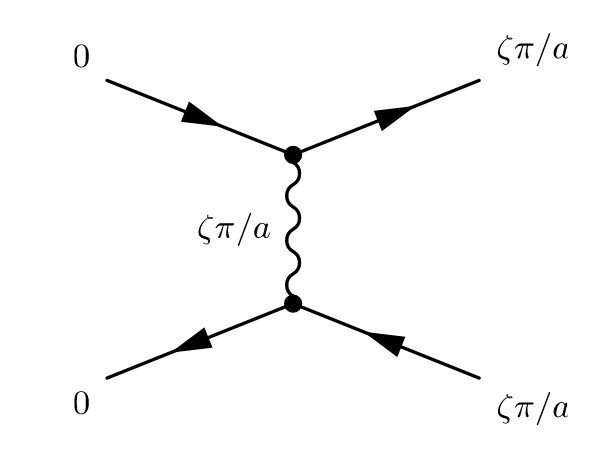
\includegraphics[width=
   0.45\textwidth]{images/tastemixing.jpg}
  \end{center}
  \caption{Taste mixing at tree level.}
  \label{fig:tastemixing}
\end{figure}

Step 2 above is the guiding principle for the action we use in our study, the Highly Improved Staggered Quark action (HISQ). 
\\ \\
Interaction between different tastes ("taste mixing") is dominated by the process in fig. \ref{fig:tastemixing}. In HISQ, this is suppressed by modifying the gauge fields in such a way as to minimize the coupling between a gluon with momentum ${\pi/a}$ and the fermions, in other words, minimize the vertices in fig. \ref{fig:tastemixing}. To this end, one can change the action so that fermions only couple to \textit{smeared} gauge links, in which high frequency exitations have been removed. \\ \\
Define the first and second covariant derivative operators:
\begin{align}
	\nonumber
	\delta_{\rho}U_{\mu}(x) & \equiv {1\over a} \big( U_{\rho} (x) U_{\mu} (x + a\hat{\rho}) U_{\rho}^{\dagger}(x+a\hat{\mu}) \\
	& - U_{\rho}^{\dagger}(x-a\hat{\rho})U_{\mu}(x-a\hat{\rho})U_{\rho}(x-a\hat{\rho}+a\hat{\mu})\big)  \\
	\nonumber
	\delta_{\rho}^{(2)} U_{\mu}(x) & \equiv {1\over a^2} \big( U_{\rho}(x+a\hat{\rho})U^{\dagger}_{\rho}(x+a\hat{\mu}) \\
	\nonumber	
	& - 2U_{\mu}(x) \\
	& + U_{\rho}^{\dagger}(x-a\hat{\rho})U_{\mu}(x-a\hat{\rho})U_{\rho}(x - a\hat{\rho} + a\hat{\mu}) \big)
\end{align}
With this we can define the smearing operator;
\begin{align}
	\mathcal{F}_{\mu} = \prod_{\rho\neq\mu} \left( 1 + {a^2 \delta^{(2)}_{\rho}\over 4} \right)
\end{align}
HISQ uses two different smeared gauge fields defined by;
\begin{align}
	X_{\mu}(x) &\equiv \mathcal{U} \mathcal{F}_{\mu} U_{\mu}(x) \\
	W_{\mu}(x) &\equiv \left(\mathcal{F}_{\mu} - \sum_{\rho\neq\mu}{a^2(\delta_{\rho})^2\over 2} \right) \mathcal{U} \mathcal{F}_{\mu} U_{\mu}(x)
	\label{eq:gaugesmearing}
\end{align}
where $\mathcal{U}$ is a re-unitarization operator. The HISQ action can then be written as:
\begin{align}
	S_{\text{HISQ}} = \sum_{x} \bar{\psi}(x) \left( \gamma\cdot \left( \nabla_{\mu}(W) - {a^2\over 6}(1+\epsilon_{\text{Naik}})\nabla^3_{\mu}(X) \right) + m \right) \psi(x)
\end{align}
Where $\nabla_{\mu}(Z)$ is the covariant derivative \eqref{eq:lat_derivative} with gauge links repaced with $Z$. This action in fact not only removes tree level interactions like fig. \ref{fig:tastemixing}, but also all taste mixing interactions at 1-loop. The $\nabla^3_{\mu}$ term is introduced to remove "lattice artifacts", i.e. it reduces the size of $\mathcal{O}(a)$ terms in the $a\to 0$ limit of the action. In the same spirit, $\epsilon_{\text{Naik}}$ is fixed according to the constraint
\begin{align}
	\lim_{\underline{p}\to 0} {E^2(\underline{p})-m^2\over \underline{p}^2} = 1
\end{align}
where $E(\underline{p})$ obeys the dispersion relation from HISQ. The motivation for the specific smearing of the gauge fields \eqref{eq:gaugesmearing}, and more details on HISQ in general, are given in \cite{Follana:2006rc}.

\subsubsection{NRQCD}

The HISQ action is suitable for fermions in the mass range of up, down, strange and charm masses. Bottom quarks are an issue, since their mass is typically higher than the cutoff $1/a$ for computationally viable lattices, so it's dynamics cannot naively be resolved on the lattice.
\\ \\
The root of the problem is in the relativistic nature of the $b$ quark. Consider the expansion in momentum $\underline{p}^2$ of the continuum relativistic dispersion relation:
\begin{align}
	\omega = \sqrt{\underline{p}^2 + m^2} \simeq m + {\underline{p}^2\over 2m} - {\underline{p}^4\over 4m^3} + ...
	\label{eq:rel_expansion}
\end{align}
the first term (rest mass) is the source of the issue, when $m > 1/a$ the first term pushes the frequency of excitations $\omega$ over $1/a$ and it's wavelength becomes hidden between the lattice points. 
\\ \\
The solution we employ is to persue instead a non-relativistic formulation, called NRQCD \cite{Lepage:1992tx}. The leading order Lagrangian in the continuum is (\cite{DeGrand:2006zz} ch. 6.6)
\begin{align}
	\mathscr{L}^0_{NRQCD} = \psi^{\dagger}_+ \left[ i\partial_0 + {\underline{\nabla}^2\over 2m_b} \right] \psi_+.
\end{align}
$\psi_+$ is the first two components of a Dirac spinor, the second two components (the antiparticle) are not present since the dispersion relation from this Lagrangian has no antiparticle solutions.
$m_b$ is the bare mass for the $b$ quark. The NRQCD action reproduces \eqref{eq:rel_expansion} with the first term chopped out.
\\ \\
Correction terms are chosen to be all gauge-invariant terms, grouped according to powers of the quark velocity $v$. For an example of deducing such powers: 
kinetic enegry = $m_b v^2 = \int d^3x \psi_+^{\dagger} {\underline{\nabla}^2\over 2m_b} \psi_+$ $\rightarrow$ $|\underline{\nabla}|/m_b \sim v$.
\\ \\
Annother benefit of NRQCD is that it does not suffer from a doubling problem, since the doubling problem is a purely relativistic issue (the doubling symmetry requires 4 component spinors for $\gamma$ matrices to act on, see appendix \ref{sec:doublingprob}). 
\\ \\
The form of the action allows propagators $M^{-1}[U]$ to be computed using a simple recursion relation
\begin{align}
	M_b^{-1}(\underline{x},t+1)[U] = e^{-aH}[U] M^{-1}_b(\underline{x},t)[U] 
\end{align}
which is numerically very fast. In the interest of numerical stability, the time evolution operator is re-cast as
\begin{align}
	e^{-aH} = \left(1 - {a\delta H\over 2}\right)\left(1-{aH_0\over 2 n}\right)^n U_0^{\dagger}(\underline{x},t) \left(1 - {aH_0\over 2n}\right)^n \left(1-{a\delta H\over 2}\right)
\end{align}
where $n$ is an arbitrary integer (chosen in our study to be $n=4$), and the Hamiltonian has been broken up into a leading part $H_0$ and correction $\delta H$. We use the $\mathcal{O}(\alpha_s v^4)$ corrected NRQCD Hamiltionian:
\begin{align}
	aH_0 =& - {\nabla^{(2)}\over 2am_b} , \\
	\nonumber
	a\delta H =& - c_1 {(\nabla^{(2)})^2 \over 8 (am_b)^3} + c_2{ i\over 8(am_b)^2} ( \underline{\nabla}\cdot \underline{\tilde{E}} - \underline{\tilde{E}}\cdot \nabla) \\
	\nonumber
	& - c_3 {1\over 8(am_b)^2} \sigma\cdot ( \underline{\nabla}\times\underline{\tilde{E}} - \underline{\tilde{E}}\times\underline{\nabla}) \\
	\nonumber
	& - c_4 {1\over 2am_b} \sigma\cdot \underline{\tilde{B}} + c_5 {\nabla^{(4)}\over 24 am_b} \\
	& - c_6 {(\nabla^{(2)})^2\over 16n (am_b)^2}
\end{align}
where $\nabla^{(2)}$ is the second lattice derivative, $\underline{\tilde{E}}$ and $\underline{\tilde{B}}$ are the chromoelectric and chromomagnetic fields, the expression for these in terms of gauge links are given in \cite{Gray:2005ur}. The coefficients $\{c_i\}$ are fixed by matching lattice NRQCD to continuum QCD up to 1-loop (thus is the quoted $\mathcal{O}(\alpha_s)$ correction).
\\ \\
Once the propagator for the 2-component non-relativistic $b$ quark has been found, it must be transformed back into a 4-component spinor. This is done by the inverse Fouldy-Wouthuysen transformation \cite{PhysRev.78.29}:
\begin{align}
	\psi(x) = e^{-{\underline{\gamma}\cdot\underline{\nabla}\over 2m_b}}\binom{\psi_+(x)}{0}
	\label{eq:FoldyWoldy}
\end{align}

\subsection{Correlation Functions from HISQ propagators and random walls}

\subsubsection{Preliminaries}
The full set of spin-mixing matrices can be labelled according to
\begin{align}
	\gamma_n = \prod_{\mu} \left( \gamma_{\mu} \right)^{n_{\mu}} \quad n_{\mu} = \mathbb{Z}_2
\end{align}
There are 16 such matrices representing corners of the hypercube. As $\gamma_{\mu}^2=1$, one can also use a general site vector $x_{\mu}$ to label the matrix, then $\gamma_x = \gamma_n$ where $n_{\mu} = x_{\mu} \mod 2$. One can show that for any $x$; $\gamma_x^{\dagger} \gamma_x = 1$.
\\ \\
Naive quarks $\psi(x)$ can be transformed into staggered quarks $\chi(x)$ via $\psi(x) = \gamma_x \chi(x)$. Then, Naive quark propagators (inverse Dirac operators) become
\begin{align}
	G_{\psi}(x,y) = \gamma_x\gamma^{\dagger}_y G_{\psi}(x,y)
\end{align}
By conjugating both sides and using $\gamma_5$-hermiticity $G^{\dagger}_{\psi}(y,x) = \gamma_5 G_{\psi}(y,x)\gamma_5$ it can be shown that
\begin{align}
	\label{eq:Gconj}
	G_{\psi}(x,y) = \phi_5(x)\phi_5(y) G^{\dagger}_{\psi}(y,x)
\end{align}
where $\phi_5(x) = (-1)^{\sum_{\mu} x_{\mu}}$.
\subsubsection{2pt correlation functions}
We will break down the correlation function to see what quantities must be computed by the simulation. Consider the generic 2-point correlator:
\begin{align}
	C(x,y) &= \langle \Phi^{\dagger}_X(x) \Phi_Y(y) \rangle_{\psi,U} \quad , \quad \Phi_X(x) = {1\over 4}\bar{\psi}_a(x) \gamma_X \psi_b(x) \\
	&= {1\over 16}\langle tr_{c,s} \gamma_X G_{a,\psi}(x,y) \gamma_Y G_{b,\psi}(y,x) \rangle_U \\
	&= {1\over 16}tr_s \left( \gamma^{\dagger}_x \gamma_X \gamma_x \gamma_y^{\dagger} \gamma_Y \gamma_y \right)
	\langle tr_c \left( G_{a,\chi}(x,y) G_{b,\chi}(y,x) \right) \rangle_U
\end{align}
$tr_s$ is a trace over spin and $tr_c$ is over colour. To deal with the spin trace, define the family of phases $\{\phi_X(x)\}$ according to
\begin{align}
	\gamma^{\dagger}_x\gamma_X\gamma_x = \phi_X(x) \gamma_X
\end{align}
for example, if $X=5$, then $\gamma^{\dagger}_x\gamma_5\gamma_x = (-1)^{\sum_{\mu}x_{\mu}} \gamma^{\dagger}_x\gamma_x \gamma_5 = \phi_5(x) \gamma_5$. The map from $X$ to $\phi_X$ is structure preserving, i.e. if $\gamma_X=\gamma_A\gamma_B$, then $\phi_X(x)=\phi_A(x)\phi_B(x)$. The spin trace becomes $\phi_X(x)\phi_Y(y) tr_s\left( \gamma_X \gamma_Y \right)$. The will vanish unless $Y=X$, as one would expect physically for the correlation function. We end up with
\begin{align}
	C(x,y) = {1\over 4} \phi_X(x)\phi_X(y) \langle tr_c G_{a,\chi}(x,y) G_{b,\chi}(y,x) \rangle_U
\end{align}
It is useful in the simulation to replace $G_{b,\chi}(y,x)$ with it's conjugate via \eqref{eq:Gconj}, resulting in
\begin{align}
	C(x,y) = {1\over 4} \phi_{5X}(x)\phi_{5X}(y) \langle tr_c G_{a,\chi}(x,y) G^{\dagger}_{b,\chi}(y,x) \rangle_U
\end{align}
where $\phi_{5X}(x) = \phi_5(x)\phi_X(x)$. To obtain the correlation function of a meson in an eigenstate with momentum ${\underline{p}}$, the above must be replaced with
\begin{align}
	C_{\underline{p}}(t_0,t) &= {1\over L^3} \sum_{\underline{x},\underline{y}} e^{i\underline{p}\cdot(\underline{x}-\underline{y})}
	C(\underline{x},t_0;\underline{y},t) \\
	&= {1\over 4 L^3} \sum_{\underline{x},\underline{y}} e^{i\underline{p}\cdot(\underline{x}-\underline{y})} \phi_{5X}(x)\phi_{5X}(y) \langle tr_c G_{a,\chi}(x,y)G^{\dagger}_{b,\chi}(y,x)\rangle_U,
\end{align}
where it is understood that $x_0=t_0$ and $y_0=t$. In order to evaluate this function, the simulation must perform inversions to create $G_{a/b,\chi}(x,y)$ for each $x$ and $y$, so $2\cdot$Vol$^2$ operations. This is prohibitively expensive. The number of inversions can be reduced using {\it{random wall sources}}. Define
\begin{align}
	P^{t_0}_{a,\underline{p},X}(y) \equiv {1\over \sqrt{L^3}} \sum_{\underline{x}} e^{i\underline{p}\cdot (\underline{x}-\underline{y})} \phi_{5X}(\underline{x},t_0) \xi(\underline{x}) G_{a,\chi}(\underline{x},t_0;y),
\end{align} 
where $\xi(\underline{x})$ is a random field of colour vectors, varying with $U$. This has the property
\begin{align}
	\langle f(\underline{x},\underline{x}') \xi^*(\underline{x}')\xi(\underline{x})\rangle_U = \delta_{\underline{x},\underline{y}} \langle f(\underline{x},\underline{y}) \rangle_U.
\end{align}
Using this property it can be shown that the correlator can be build instead according to
\begin{align}
	C(\underline{x},t_0;\underline{y},t) \simeq {1\over 4} \sum_{\underline{y}} \phi_{5X}(y) \langle tr_c P^{t_0}_{a,\underline{p},X}(\underline{y},t)P^{t_0,\dagger}_{b,\underline{0},1}(\underline{y},t)\rangle_U
	\label{eq:tietogether}
\end{align}
Now all the simulation has to do is compute $P^{t_0}_{a/b}(y)$ for general $y$, so $2\cdot$Vol operations, a reduction by a factor of Vol. 
\\ \\
In the MILC code, "sources" are first created (the fields $\phi_{5X}(\underline{x},t_0) \xi(\underline{x})$), then the objects $P^{t_0}(y)$ (referred to as "propagators") are generated from them. Any extra factors dependant on $y$ (this is useful for "smeared" propagators, see {\color{red}?}) can be multiplied in. The resulting object $f(y)\cdot P^{t_0}(y)$ is referred to as a "quark". Finally, two of these quarks can be "tied together" according to \eqref{eq:tietogether}, to produce correlation functions. The sources are chosen to be on some single timeslice $t_0$, resulting in a value for $C(t_0,t)$ at each $t$. 

\subsubsection{3-point correlators}

The above discussion can be generalized to $3-$(or $N-$)point correlation functions using {\it{extended sources}}. Consider a 3-pt correlator encoding the form-factors of a semileptonic decay from meson $X$ to meson $Z$, via a current $J$. We start by evaluating
\begin{align}
	C(x,y,z) = \langle \Phi^{\dagger}_X(x) J(y) \Phi_Z(z) \rangle_{\psi,U} \quad , \quad \Phi_X(x) &= {1\over 4} \bar{\psi}_b(x) \gamma_X \psi_s(x) \\
	\nonumber
	J(y) &= \bar{\psi}_b(y)\gamma_J\psi_a(y) \\
	\nonumber
	\Phi_Z(z) &= {1\over 4}\bar{\psi}_a(z)\gamma_Z \psi_s(z)
\end{align}
in the same way as before:
\begin{align}
	C(x,y,z) &= {1\over 16} tr_s\left( \gamma^{\dagger}_x \gamma_X \gamma_x \gamma^{\dagger}_y \gamma_J \gamma_y \gamma^{\dagger}_z \gamma_Z \gamma_z \right) \langle tr_c G_{b,\chi}(x,y) G_{a,\chi}(y,z) G_{s,\chi}(z,x)\rangle_U \\
	&= {1\over 4} \phi_{5X}(x) \phi_J(y) \phi_{5Z}(z) \langle tr_c G_{b,\chi}(x,y) G_{a,\chi}(y,z) G^{\dagger}_{s,\chi}(z,x) \rangle_U
\end{align}
We have assumed that $tr_s \gamma_X\gamma_J\gamma_Z = 4$, requiring that each gamma matrix in this combination has a partner and therefore cancels. In any other situation the trace would vanish. For example, if the current is a temporal vector $J=0$, and the two mesons represent pseudoscalars, one of the meson operators must have a $\gamma_0$, i.e. one could choose $\gamma_X=\gamma_0\gamma_5, \gamma_Z=\gamma_5$. {\color{red}why is it ok to have a non-goldstone for $X$?}
\\ \\
Putting $X$ into an eigenstate of zero momentum, and $Y$ into an eigenstate of momentum $\underline{p}$, we get
\begin{align}
	C_{\underline{p}}(t_0,t,T) = {1\over 4 L^3} \sum_{\underline{x},\underline{y},\underline{z}} e^{i\underline{p}\cdot(\underline{y}-\underline{z})} \phi_{5X}(x) \phi_J(y) \phi_{5Z}(z) \langle tr_c G_{b,\chi}(\underline{x},t_0;\underline{y},t) G_{a,\chi}(\underline{y},t,\underline{z},T) G^{\dagger}_{s,\chi}(\underline{z},T;\underline{x},t_0) \rangle_U
	\label{eq:3ptfullexpr}
\end{align}
This can be built by first creating propagators for the $b$ and $s$ quarks: $P^{t_0}_{b,\underline{0},X}(y)$,$P^{t_0}_{s,\underline{0},1}(z)$. Then, build the $a$ propagator using an extended source, i.e.:
\begin{align}
	P^T_{a,\underline{p},ext}(y) = \sum_{\underline{z}} P^{t_0}_{s,\underline{0},1}(\underline{z},T) \phi_{5Z}(\underline{z},T) G_{a,\chi}(\underline{z},T;y)
\end{align}
Then, by plugging $P^{t_0}_{b,\underline{0},X}(y)$ and $P^T_{a,\underline{p},ext}(y)$ into the MILC tie-together defined by \eqref{eq:tietogether},one ends up evaluating \eqref{eq:3ptfullexpr}.

\subsection{Fitting Correlation Functions}
\label{sec:fitting}

Once a correlation function like the in \ref{sec:correlators} has been computed, we can extract physics from it, namely the mass and decay constant of the meson we are studying. In practice the meson creation operators defined above are fourier transformed
\begin{align}
	\Phi(\underline{k},t) = \sum_{\underline{x}} e^{-i\underline{k}\cdot\underline{x}} \Phi(\underline{x},t)
\end{align}
which serves to change \eqref{eq:av_gauge} into 
\begin{align}
	C_{\underline{k}}(t) = {1\over N} \sum_i \sum_{\underline{x},\underline{y}} e^{-i\underline{k}\cdot(\underline{x}-\underline{y})} \text{ Tr}\left[\text{ } M^{-1}_b(\underline{y},t;\underline{x},0)[U_i] \gamma_5 M^{-1}_d(\underline{x},0;\underline{y},t)[U_i] \gamma_5 \text{ }\right]
	\label{eq:correlator}
\end{align}
\eqref{eq:correlator} is computed for many $t$ values with a lattice calculation following the principles detailed above. One performs a least-squares fit of 
this to a theoretically motivated function of $t$. To derive such a function,
first construct a complete set of momentum $\underline{k}$ states with quantum numbers matching the meson:
\begin{align}
 1 = \sum_{n=0} {1\over 2E^r_n} | \lambda_n \rangle \langle \lambda_n |.
\end{align}
Where $E^r_n = \sqrt{ M_n^2 + \underline{k}^2}$ are the relativistic energies of each state. Inserting this into the correlation function, and moving from the Heisenberg to Schroedinger picture;
\begin{align}
	C_{\underline{k}}(t) &= \sum_{n=0} {1\over 2E^r_n} \langle 0 | e^{Ht} \Phi(\underline{k},0) e^{-Ht} | \lambda_n \rangle \langle \lambda_n | \Phi^{\dagger}(\underline{k},0) | 0 \rangle
	\nonumber
	\\ &= \sum_{n=0}  \left( {\langle 0 | \Phi(\underline{k},0) | \lambda_n \rangle \over \sqrt{2E^r_n}} \right) \left( {\langle \lambda_n | \Phi^{\dagger}(\underline{k},0) | 0 \rangle \over \sqrt{2E^r_n} } \right) e^{-E^l_n t}
	\nonumber
	\\ & \equiv \sum_{n=0} |a_n|^2 e^{-E^l_n t}.
	\label{eq:multiexponential}
\end{align}
The fit results in a determination of the parameters $a_n$, and $E^l_n$. Since the lowest energies dominate the function at late times, one can afford to truncate the sum over $n$ to some tractable range, in our case $n\in[1,6]$. We interpret $|\lambda_0\rangle$ to be the ground state of the meson we are studying. The exponential decays mean the fit function is dominated by the ground state at large $t$, and subsequent excited states become less important as $E^l_n$ increases. Hence by only including $C_{\underline{k}}(t)$ at suitably large $t$ values, we can affort to truncate the sum in $n$. In our fits we chose $n=6$.
\\ \\
We maintain a distinction between $E^l$ and $E^r$, since for example in simulations involving NRQCD quarks these differ. If this is not an issue, as is the case with HISQ, one can compute the correlation function at zero momentum $C_{\underline{0}}(t)$, then fit it to find the parameter $E^l_0$, which will equal the meson's mass $M$. Noting the definition of a meson decay constant $f$: $\langle 0 | J_0 | \text{Meson}(\underline{k}=0) \rangle = M f$, where $J_0$ is a temporal current with the same quantum numbers as the meson, we can see that the fit parameters $a_n$ at zero momentum are related to the meson's decay constant via
\begin{align}
	f = \sqrt{2\over M} a_0
\end{align}
Hence the fit can also be used to extract decay constants.
\\ \\
The above discussion can be straightforwardly generalized to 3-point correlation functions, from which we are able to extract quantities like the hadronic transition amplitudes $H_{\mu} = \langle M_{q_1\bar{q_3}} | J_{\mu}^{q_1\bar{q}_2} | M_{q_2\bar{q}_2} \rangle$ from sec. \ref{sec:cp}. Specifically the quantity we require in order to deduce the $B_{s}\to D_{s} l\nu$ form factors is $\langle D_{s} | V_{\mu} | B_{s} \rangle$, where $V_{\mu}=\bar{c}\gamma_{\mu} b$. 
\\ \\
The generalization of the above for 3pt functions is summarized here:
\begin{align}
	C_3(t,T) &= \int \mathcal{D}\psi \mathcal{D}\bar{\psi} \mathcal{D}U \left(\text{ } \Phi_{D_s}(\underline{0},0) V_{\mu}(-\underline{p},t) \Phi_{B_s}^{\dagger}(\underline{p},T) \text{ }\right) e^{-S[\psi,\bar{\psi},U]} \\
	&\simeq {1\over N} \sum_i \sum_{\underline{x},\underline{y},\underline{z}} e^{-i\underline{p}\cdot (\underline{y}-\underline{z})} \text{ Tr}\left[\text{ } M^{-1}_b(\underline{x},0;\underline{y},t)[U_i] \gamma_{\mu} M^{-1}_c(\underline{y},t;\underline{z},T)[U_i]\gamma_5\gamma_5 M_s^{-1\dagger}(\underline{z},T;\underline{x},0)[U_i]  \text{ }\right] \\	
	&= \sum_{n,m}  \left( {\langle 0 | \Phi_{D_s} | \lambda_n \rangle \over \sqrt{2E^r_n}} \right) \left({\langle \lambda_n | V_{\mu} | \lambda_m \rangle \over 2\sqrt{ E^r_n E^r_m } }\right) \left( {\langle \lambda_m | \Phi_{B_s}^{\dagger} | 0 \rangle \over \sqrt{2E^r_n} } \right) e^{-E^l_m (T-t)} e^{-E^l_n t} \\
	\nonumber
	& \equiv \sum_{n,m} a_{D_s,n} V_{nm} a^*_{B_s,m} e^{-E^l_m (T-t)} e^{-E^l_n t}.
	\label{eq:3ptfitfunction}
\end{align}
$C(t,T)$ is computed at different values of $t$ and $T$, then a least-squares fit is performed to the fit function \eqref{eq:3ptfitfunction}. $a_n$ will vanish for states $|\lambda_n\rangle$ which have different quantum numbers to $\Phi_{B_s}$, and similarly for $b_m$ and $\Phi_{D_s}$. Non-zero $a_n$'s will match the analagous parameters extracted from fitting a 2pt function $\langle \Phi_{B_s}^{\dagger} \Phi_{B_s} \rangle$, similarly for $b_n$'s and $\Phi_{D_s}$. This carries on to the energies, $\{E^l_n\}$ is the spectrum for the $D_s$ meson, and $\{E^l_m\}$ is the spectrum for the $B_s$. Therefore, we compute and fit the appropriate 2pt functions to deduce the parameters $\{a_n\}$,$\{b_m\}$,$\{E^l_n\}$. Then, fitting $C_3(t,T)$ results in an accurate determination of the remaining free parameters, $V_{nm}$. This set contains the quantity we need, recoginising that:
\begin{align}
	V_{00} = {\langle D_s | V_{\mu} | B_s \rangle \over 2\sqrt{E^{B_s} E^{D_s} } }
\end{align}

\subsection{Renormalization of Currents}
\label{sec:renormalization}

Once one has computed a matrix element from a lattice calculation, it needs to be translated into a continuum regularization scheme. Suppose we have some bare operator $\mathcal{O}_0$, we expect this to be related to the renormalized operator in $\overline{MS}$ at scale $\mu$, $\mathcal{O}^{\overline{MS}}(\mu)$, via
\begin{align}
	\mathcal{O}^{\overline{MS}}(\mu) = Z^{\overline{MS}}(\mu) \mathcal{O}_0.
\end{align}
Similarly, in a lattice regularization,
\begin{align}
	\mathcal{O}^{\text{lat}}(1/a) = Z^{\text{lat}}(1/a) \mathcal{O}_0.
\end{align}
Hence we expect a multiplicative factor between the lattice matrix elements, and the continuum $\overline{MS}$ ones:
\begin{align}
	\langle \mathcal{O} \rangle^{\overline{MS}} = \mathcal{Z}(\mu,1/a) \langle \mathcal{O} \rangle^{\text{lat}}
\end{align}
where $\mathcal{Z}(\mu,1/a) = Z^{\overline{MS}}(\mu)/Z^{\text{lat}}(1/a)$. These "matching factors" $\mathcal{Z}$ can be deduced by equating observables calculated in both lattice QCD and continuum (appropriately regularized) QCD, producing equations which can be solved for $\mathcal{Z}$. The lattice side of the calculation can be done either through lattice perturbation theory ("perturbative matching"), or through a simulation ("non-perturbative matching").
\\ \\
It is a well-known result that conserved (or partially conserved) currents do not receive any renormalization in any scheme, i.e. $Z^{\text{any}}=1$ ("absolutely normalized").
\\ \\
In principle this is of great help, since the currents we are calculating, namely $V_{\mu}$, are partially conserved, so we are not required to include any matching factors. However in practice, this is complicated by the fact that the conserved current in the lattice theory is often computationally difficult or impossible to compute. For example, in NRQCD, the partially conserved current corresponding to $SU(N)_V$ is an infinite sum in $1/m_b$ where $m_b$ is the bottom mass. The corresponding current in HISQ is also the sum of a large number of operators. This can be interpreted as a mixing in the renormalization:
\begin{align}
	\langle \mathcal{O}_i \rangle^{\overline{MS}} = \mathcal{Z}_{i,j} \langle \mathcal{O}_j \rangle^{\text{lat}}
\end{align}
In practice, lattice calculations often use only the dominant operators that contribute to the conserved current. Since these will be "close" to the conserved current, one can expect the matching factor to only be a small deviation from unity, and the more sub-dominant operators you add, the overall matching factor should tend towards one.

%-------------------------------------------------------------------------------------

\section{Calculation Details}
\label{sec:deets}

\subsection{Lattice Setup}


\begin{table}
\begin{center}
 \begin{tabular}{||c c c c c c c c||}
 \hline
 Set & $a/\text{fm}$ & $am_l$ & $am_s$ & $am_c$ & $L_x/a$ & $L_t/a$ & $N_{\text{cfg}}$ \\ [0.5ex] 
 \hline\hline
 1 & 0.1474(15) & 0.013 & 0.065 & 0.838 & 16 & 48 & 1020 \\ [1ex]
 2 & 0.1219(9) & 0.0102 & 0.0509 & 0.635 & 24 & 64 & 1053 \\ [1ex]
 3 & 0.0884(6) & 0.0074 & 0.037 & 0.440 & 32 & 96 & 1008 \\ [1ex]
 \hline
\end{tabular}
\caption{Parameters for gauge ensembles \cite{Bazavov:2012xda}.
$a$ is the lattice spacing, deduced from a study of the
$\Upsilon$-$\Upsilon'$ splitting \cite{Dowdall:2011wh}. $L_x$ is the spacial extent and $L_t$ the
temporal extent of the lattice. The masses of up, down, stange and
charm quarks included in the sea are given as the dimensionless quantity $am$.
Up and down quarks are taken to have the same mass, $am_l$. $N_{\text{cfg}}$ is the number of configurations in the ensemble. We calculate propagators from 16 time sources on each ensemble to increase statistics. \label{table:ensembles}}
\end{center}
\end{table}

\begin{table}
\begin{center}
 \begin{tabular}{||c c c c c c c c c c||}
 \hline
 Set & $am_s$ & $am_c$ & $am_b$ & $u_0$ & $\epsilon_{\text{Naik}}$ & $c_{1,6}$ & $c_5$ & $c_4$ & $\{T\}$ \\ [0.5ex] 
 \hline\hline
 1 & 0.0705 & 0.826 & 3.297 & 0.8195 & -0.3449 & 1.36 & 1.21 & 1.22 & 8, 11, 14 \\ [1ex]
 2 & 0.0541 & 0.645 & 2.66 & 0.8340 & -0.2348 & 1.31 & 1.16 & 1.20 & 9, 12, 15 \\ [1ex]
 3 & 0.0376 & 0.450 & 1.91 & 0.8525 & -0.1256 & 1.21 & 1.12 & 1.16 & 14, 19, 24 \\ [1ex]
 \hline
\end{tabular}
\caption{Parameters used in our calculation. $am_s$ and $am_c$ are the bare masses of the strange, charm valence quarks, tuned in \cite{PhysRevD.91.054508}, $am_b$ is the bare mass of the valence bottom quark, tuned in \cite{Dowdall:2011wh}
$u_0$ is the 'tadpole improvement parameter' as used in \cite{Dowdall:2011wh}.
$\epsilon_{\text{Naik}}$ is the Naik parameter in the HISQ action \cite{Follana:2006rc}.
$\{c_i\}$ are the coefficients for the kinetic and chromomagnetic terms in the NRQCD action \cite{Hammant:2013sca}. $\{T\}$
is the set of temporal seperations between source ($B_s$ creation operator) and sink ($D_s$ anihilation operator). \label{table:quarkmasses}
}
\end{center}
\end{table}

We follow a largely similar approach to the recent $B\to Dl\nu$ and $B_s\to D_sl\nu$ calculations in \cite{Na:2015kha} and \cite{Monahan:2017uby}.
\\ \\
Table \ref{table:ensembles} gives details of the ensembles used in this study. These are taken from the MILC HISQ ensembles \cite{Bazavov:2012xda}. They are generated by MCMC with the distribution given in \eqref{eq:MCweight}, where $M$ is the Dirac operator for the HISQ action. They take into accound up, down, strange and charm quarks, assuming the contribution from higher mass quarks in the sea to be negligable.
\\ \\
Following the procedure discussed in section \ref{sec:correlators}, first we must compute 2-point correlators for the $B_s$ and $D_s$. In both cases we use \textit{smeared} creation operators:
\begin{align}
	\Phi^{\alpha}(\underline{k},t) = \sum_{\underline{x},\underline{x'}} e^{-i\underline{k}\cdot\underline{x}} \text{ } \bar{\psi}_1(\underline{x'},t)\phi^{\alpha}(\underline{x}'-\underline{x}) \gamma_5 \psi_2(\underline{x})
\end{align}
where $\bar{\psi}_1$,$\psi_2$ are $\bar{b}$,$s$ for the $B_s$ and $\bar{c}$,$s$ for the $D_s$. The smearing functions $\phi^{\alpha}$ approximate the wavefunction of one quark in a potential set up by the other, giving a psuedo-realistic representation of the meson. This makes the operator $\Phi^{\alpha}$ couple stronger to the ground state of the meson, maximizing the $a_0 \propto \langle0 |\Phi^{\alpha}|\lambda_0\rangle$ parameter in the fit \eqref{eq:multiexponential} relative to the excited states $a_{n>0}$. This increases the dominance of the first term in \eqref{eq:multiexponential} resulting in better convergence of the $n$ sum, therefore a better fit and better statistics of the results.
\\ \\
For the $B_s$, we use a combination of $\phi^0(\underline{z})=\delta(\underline{z})$ ("local"), and $\phi^{1,2}(\underline{z}) \propto \text{exp}(-|\underline{z}|/r_0)$ ("smeared"), with $r_0 \simeq 2.5$fm$, 5$fm. For the $D_s$ we use one local and one smeared with $r_0\simeq2.5$fm. Correlation functions between each smearing combination is calculated, i.e. for the $D_s$, we compute 4 correlators $\langle \Phi^{0\dagger}_D\Phi_D^0 \rangle$, $\langle \Phi^{1\dagger}_D\Phi_D^0 \rangle$, $\langle \Phi^{0\dagger}_D\Phi_D^1 \rangle$, $\langle \Phi^{1\dagger}_D\Phi_D^1 \rangle$, and 9 for the $B_s$.
\\ \\
A good way to see the benefit of the smearing is by plotting the effective mass $m_{\text{eff}}(t) = \text{log}({C(t)/C(t+1)})$ against $t$ as in fig. \ref{fig:effmass}. The flatness of this as a function in $t$ shows how well it is approximated by the fit function with only the ground state (i.e. not contaminated by excited states), therefore how easily the fit will determine the ground-state energy. As can be seen, The smeared effective mass "flattens out" quicker than the local, as the smeared couples mostly to the ground state.
\\ \\
\begin{figure}
  \begin{center}
    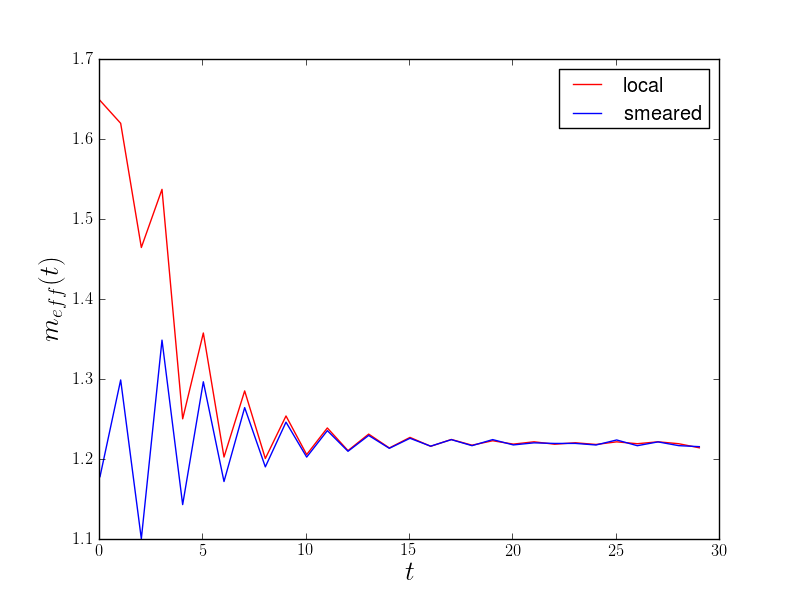
\includegraphics[width=
   0.65\textwidth]{images/EffMass_localVsSmear_Ds_coarse.png}
  \end{center}
  \caption{Effective mass of $D_s$ correlation functions, one with local $D_s$ operators $\langle\Phi^0\Phi^0\rangle$ and one with smeared $\langle\Phi^1\Phi^1\rangle$.}
  \label{fig:effmass}
\end{figure}

The 3pt correlation function calculated is $\langle \Phi^{\alpha\dagger}_{D_s} V_{\mu} \Phi^{\beta}_{B_s} \rangle$, including all smearings of the $B_s$ and $D_s$ used in the 2-point functions. We must be careful choosing the appropriate operator for $V_{\mu}$. Recall that NRQCD quarks contain an inverse Fouldy-Wouthuysen (FW) transformation \eqref{eq:FoldyWoldy}. This must be encorparated into the $V_{\mu}$ operator, since it couples to the $b$ which obeys the NRQCD action in our simulation. Hence the $V_{\mu}$ operator must be of the form
\begin{align}
	V_{\mu} = \bar{c}\gamma_{\mu}\left( 1 - {1\over 2m_b} \underline{\gamma}\cdot\underline{\nabla} + \mathcal{O}\left({1\over m_b^2}\right) \right) b 
\end{align}
where we can afford to expand the exponential in the FW transformation since $1/m_b$ is small. However, this is only a tree level result. According to the discussion in sec. \ref{sec:renormalization}, these terms require renormalization constants, and also new terms in the above expansion may appear. Therefore the full expression for the vector current that we use is (accurate to $\mathcal{O}(\alpha_s,1/m_b)$):
\begin{align}
	\nonumber
	V_{\mu} &= (1+z_0 \alpha_s)\left[ V_{\mu}^{(0)} + (1 + z_1 \alpha_s) V_{\mu}^{(1)} + z_2 \alpha_s V_{\mu}^{(2)} \right] \\
	\nonumber
	& V_{\mu}^{(0)} = \bar{c}\gamma_{\mu} b \\
	\nonumber
	& V_{\mu}^{(1)} = -{1\over 2m_b} \bar{c} \gamma_{\mu}\underline{\gamma}\cdot\underline{\nabla} b \\
	\nonumber
	& V_{\mu}^{(2)} = -{1\over 2m_b} \bar{c} \gamma_{\mu}\underline{\gamma}\cdot\underline{\overleftarrow{\nabla}} b \\
	\label{eq:currentcorrections}
\end{align}
The coefficients $\{z_i\}$ are set by a matching procedure between the HISQ/NRQCD currents and continuum QCD in \cite{Monahan:2012dq}. We calculate correlation functions $\langle \Phi_{D_s} V^{(i)}_{\mu} \Phi_{B_s}\rangle$ for each current and combine them after the fitting procedure.

\subsection{Correlator Fits}

2-point correlation functions are then fitted as in sec. \ref{sec:fitting}. The fit function we use is modified a little from \eqref{eq:multiexponential}, we use:
\begin{align}
	\nonumber
	C^{\alpha\beta}(t) &= \sum_{n} a^{\alpha*}_n  a^{\beta}_n ( e^{-E^l_n t} - se^{-E^l_n(T-t)} )\\
	& + \sum_{n} a^{'\alpha*}_n a^{'\beta}_n (-1)^t ( e^{-E^{'l}_n t} - se^{-E^{'l}_n(T-t)} )
	\label{eq:2ptcorrelator_real}
\end{align}
Firstly, the parameters $\{a_n\}$ must vary between source and sink to account for the different operators. Secondly, the periodicity of the lattice in the time direction means an extra exponential term is required, but not in the case of the $B_s$ since NRQCD quarks do not experience the periodicity of the lattice. Hence $s$ is set to 0 for the $B_s$ correlator and 1 for the $D_s$. $T$ is the time extent of the lattice. The second term is to account for the so-called "oscillating state", which is in fact the $\zeta=(1,0,0,0)$ doubler fermion appearing due to the doubling in the HISQ action (see sec. \ref{eq:doubling}). No other doublers contribute, since $\Phi_{\underline{k}}$ has a 3-momentum fixed at $\underline{k}$, which we always take to be small relative to $\pi/a$, hence does not couple to the states at $k\sim(0,\pi/a,0,0)$, $k\sim(0,0,\pi/a,0)$ etc. However, $\Phi_{\underline{k}}$ can couple to arbitrarily high energy states, so the $k\sim(\pi/a,0,0,0)$ doubler contributes. The second term in \eqref{eq:2ptcorrelator_real} is justified by performing the doubling operation $\mathcal{B}_0$ defined in \eqref{eq:multiexponential}, the quark fields in $\Phi_{\underline{k}}$ which obey the HISQ action. See appendix G of \cite{Follana:2006rc} for details.
\\ \\
We use the \textit{CorrFitter} package \cite{CorrFitter} for performing Baysian least-squares fitting to the correlation functions. The package employs the trust region method of least-squares fitting. The fits require priors for each of the fit parameters. The "amplitude" parameters $a_{n,B_s/D_s}^{\alpha}$ are given priors of $0.1(1.0)$, thus inserting only the assumption that they are of $\mathcal{O}(1)$. The ground state energies are given priors motivated by the meson masses, and excited state energies are given loose, evenly spaced priors with ~600MeV between each level.
\\ \\
2-point correlation functions for $B_s$ and $D_s$ are fit to \eqref{eq:2ptcorrelator_real}, resulting in $a^{\alpha}_{n,B_s/D_s}$,$E^l_{n,B_s/D_s}$. Since the HISQ action is fully relativitstic, $E^l_{0,D_s}$ at $\underline{k}=0$ can be interpreted as the $D_s$ meson mass. The same cannot be done for the $B_s$. The decay constants for $B_s$ and $D_s$ can be deduced from $a^0_{0,B_s}$ and $a^0_{0,D_s}$, since $\Phi^0_{B_s,D_s}$ are also temporal axial currents. This is a good avenue for consistency checks, we compared $M_{D,s}$,$f_{D_s}$ and $f_{B_s}$ to those computed in \cite{Colquhoun:2015oha},\cite{Monahan:2017uby} amongst others, and found them to be consistent (modulo small shifts we can reasonably expect due to differing choices of bare quark masses).
\\ \\
We now discuss fitting the 3-point correlation functions. The same considerations as those that went into \eqref{eq:2ptcorrelator_real} lead us to our 3-point fit function:
\begin{align}
	\nonumber
	C^{\alpha\beta}_3(t,T) =& \sum_{k,m} \big( a_{k,D_s}^{\alpha} V^{nn}_{km} a_{m,B_s}^{*\beta} e^{-E^l_m t} e^{-E^l_k (T-t)} \\
	\nonumber
	& + a_{k,D_s}^{\alpha} V^{no}_{km} a_{m,B_s}^{'*\beta} e^{-E'^l_m t} e^{-E^l_k (T-t)} \\
	\nonumber
	& + a_{k,D_s}^{'\alpha} V^{on}_{km} a_{m,B_s}^{*\beta} e^{-E^l_m t} e^{-E'^l_k (T-t)} \\
	& + a_{k,D_s}^{'\alpha} V^{oo}_{km} a_{m,B_s}^{'*\beta} e^{-E'^l_m t} e^{-E'^l_k (T-t)} \big)
	\label{eq:3ptcorrelator_real}
\end{align}
The 2-point and 3-point correlators are fit simultaniously, according to fit functions \eqref{eq:2ptcorrelator_real} and \eqref{eq:3ptcorrelator_real}. The parameters involved in the 2pt fits are mostly fixed by the data in the 2pt correlation functions, so the fit can use most of the data in the 3pt correlation functions to determine the transition amplitudes $V^{ab}_{km}$. This is carried out for each $B_s$ and $D_s$ smearing, each direction $\mu$ and each current correction $i$ of the vector current $V^{(i)}_{\mu}$.
\\ \\
In this large 2pt/3pt fit, there is a huge $\chi^2$ manifold with many local minema, and it is crucial to impose strong priors in order to ensure the fit finds the true minemum. Priors for ground state 2-point amplitudes and energies $a_{0,B_s/D_s}^{\alpha}$,$E^l_{0,B_s/D_s}$ are taken to be the results from individual fits of the 2-point functions, with the errors expanded by a factor of 2. The excited state amplitudes and energies are given the same priors as in the 2-point fits. The transition amplitueds $V^{ab}_{km}$ are given the prior 0.1(1.0), assuming it to be $\mathcal{O}(1)$.
\\ \\
Finally, we end up with the sought-after parameters $V_{00}^{nn}$ representing $V_{\mu}^{(i)}$, via the relation
\begin{align}
	\langle D_s | V^{(i)}_{\mu} | B_s \rangle =  2\sqrt{M^{B_s} E^{D_s}} V_{00}^{nn} |_{V=V_{\mu}^{(i)}\text{in simulation}}
\end{align}
We have asserted the ground state of $B_s$ to be it's mass, but not the $D_s$, as we give $D_s$ spacial momenta in the calculation (to be expanded on in the next section). Then, the full vector currents $\langle D_s | V^{(i)}_{\mu} | B_s \rangle$ can be build from a linear combination of these according to \ref{eq:currentcorrections}.

\subsection{Deduction of Form Factors}

We wish to use these currents to deduce the $B_s\to D_s l\nu$ form factors discussed in section \ref{sec:formfactors} over the full $q^2$ range. To this end, the above procedure to compute $\langle D_s | V^{(i)}_{\mu} | B_s \rangle$ is repeated while giving the $D_s$ meson a range of different spacial momenta. We chose spacial momentum $\underline{p} = |\underline{p}|(1,1,1)$, in this each direction is equivilant, and it allows us to average $V_{\mu}$ over the 3 spacial directions, reducing work in the fit and increasing the statistics of the averaged current $V_k \equiv \sum_{i=1}^3 V_i / 3$.
\\ \\
As discussed in appendix \ref{sec:signalnoise}, the most accurate results will come from $|\underline{p}| = 0$, then the correlators become noise-dominated as one increases $|\underline{p}|$ towards $|\underline{p}|_{\text{max}}$. Hence, the approach is to start at the $|\underline{p}|=0$ end and move up in momentum, monitoring statistical errors as you go. So far we have performed runs for $|a\underline{p}| = 0,0.30,0.45$ on the fine ensemble, and $|a\underline{p}|=0,0.25,0.50$ on the coarse ensemble. Statistical errors have not yet become uncontrollable at these momenta, but from experience of previous calculations, they are expected to become problematic at $|a\underline{p}| \sim 0.7$. 
\\ \\
With values for $\langle D_s | V_{\mu} | B_s \rangle$ at varying $\underline{p}$ therefore varying $q^2$, we can perform a fit of this data in order to extract $f_{0,+}(q^2)$ via \eqref{eq:formfactors}. To do the fit, we need some anzats for the functional form of $f_{0,+}(q^2)$. We use the BCL parameterization \cite{PhysRevD.79.013008}. This involves first reparameterizing $q^2$ to 
\begin{align}
	z(q^2) = {\sqrt{t_+ - q^2} - \sqrt{t_+ - t_0} \over \sqrt{t_+ - q^2} + \sqrt{t_+ - t_0} }
\end{align}
where we take $t_0 = t_+( 1 - \sqrt{1 - t_-/t_+})$, and $t_{\pm} = (M_{B_s} \pm M_{D_s})^2$, as in \cite{Hill:2006ub}. $z(q^2)$ has a very small magnitude throughout the entire $q^2$ range, in our case $|z|_{\text{max}} \sim 0.032$. We can then accurately model $f_{+,0}$ as a series expansion in $z$:
\begin{align}
	f_{0,+}(q^2) = {1\over P_{0,+}(q^2)} \sum_n a^{0,+}_n z(q^2)^n
	\label{eq:zexpansion}
\end{align}
we truncate this at $z^2$, adding further terms have no effect on the fit. The so-called Blaschke factors $P(q^2)$
are defined by
\begin{align}
	P_{0,+}(q^2) = \left( 1 - {q^2\over M_{0,+}^2}\right)
\end{align}
These are required due to subthreshold poles in the crossed channel of $\langle D_s | V^{(i)}_{\mu} | B_s \rangle$, which in our case is a $W$ decay into a $B_c$ meson. The pole is located where the $W$ has the correct momentum $q^2$ to create the $B_c$, hence at $q^2=M_{B_c}$. This is not within the $q^2$ range, but can create curvature in $f_{0,+}$ that can confound the expansion in $z$. $P_{0,+}$ effectively removes this pole from the $z$ expansion.

\subsubsection{Using only Scalar and Temporal Vector Currents}

The continuum currents $V_0$ and $S$ are given by
\begin{align}
        V_0 &= (1 + \alpha_s (\eta_{0}^{V_0} - \tau_{01}^{V_0})) \times \left( J_{V_0}^{(0)} + J_{V_0}^{(1)} \right) \\  
        m_b S &= (1 + \alpha_s (\eta_{0}^{V_0} + \tau_{01}^{V_0} + C_M))\times {am_b\over a} \times \left( J_{V_0}^{(0)} - J_{V_0}^{(1)} \right)
\end{align}
The scalar current $F_0(q^2)$ can be extracted from $m_b S$ via
\begin{align}
        m_b \left(1 - {m_c\over m_b} \right) \langle D | S | B \rangle &= ( M_B^2 - M_D^2 ) F_0(q^2)
\end{align}
Once $F_0(q^2)$ is constrained, all the information in $V_0$ can be used to constrain $F_+(q^2)$:
\begin{align}
        \langle D | V_0 | B \rangle = \left( p_B^0 + p_D^0 - {{M_B^2-M_D^2}\over q^2} q^0 \right) F_+(q^2) \\
                + {{M_B^2-M_D^2}\over q^2} q^0 F_0(q^2)
                \nonumber
\end{align}
Let's write these relations as
\begin{align}
        \label{eq:scalartoff}
        m_b S & \equiv R_{S0} F_0 \\
        V_0 & \equiv R_{0+} F_+ + R_{00} F_0
\end{align}
To deduce $F_0$ we use \eqref{eq:scalartoff}, then to deduce $F_+$ via:
\begin{align}
        F_+ = {V_0 - R_{00} F_0 \over R_{0+}}
\end{align}
Close to $q^2_{\text{max}}$, there is something of a "fine tuning problem" in this equation. Consider the size of each of these terms:
\begin{align}
        \mathcal{O}(1) = {\mathcal{O}(10) - \mathcal{O}(10) \over \mathcal{O}(0.1)}
\end{align}
$V_0$ and $R_{00}F_0$ must cancel to a high precision in order to reproduce an $F_+$ of $\mathcal{O}(1)$.  The correlation between $V_0$ and $S$ is smaller than I expected, $\sim$0.5, so this does not improve much the precision of $V_0-R_{00}F_0$. Even if it did, any error in matching factors will cause a large difference between $V_0$ and $R_{00} F_0$.
\\ \\
At the moment, I am getting
\begin{align}
        F_+ \sim 10
\end{align}
at the lowest non-zero momentum point on very coarse, while we expect $F_+ \sim 1$.
\\ \\
A possible direction to go in is to define something like
\begin{align}
        \nonumber
        V_{\alpha} &\equiv V_0 - \alpha_s V_k \\
        &= (R_{00} - \alpha_s R_{k0} )F_0 + (R_{0+}-\alpha_s R_{k+})F_+ \\
        \nonumber
        &\equiv R_{\alpha 0} F_0 + R_{\alpha +} F_+
\end{align}
$V_{\alpha}$ does not contain the $V_k$ loop corrections we were worried about, but adds some information from it's leading order. Then $F_+$ can be deduced instead from
\begin{align}
        F_+ = {V_{\alpha} - R_{\alpha 0} F_0 \over R_{\alpha +}}
\end{align}
which suffers from less of a tuning problem, via this method I get
\begin{align}
        F_+ \sim 4
\end{align}
\\ \\
Flipping the sign of $J_{V_0}^{(1)}$ seems to ease this problem further, are we confident that the sign we are using is correct? With the sign flipped, we get to
\begin{align}
        F_+ \sim 2
\end{align}
Still not at a point where this is useful, but there could be other improvements to be made...

\subsection{Continuum \& Chiral Extrapolation}

The form factors $f_{0,+}(q^2)$ we deduce from the above will contain systematic errors due to 1) discretization, and 2) unphysical quark masses and mistunings. 
\\ \\
2) requires a little explaination. In lattice simulations it is computationally expedient (and sometimes neccesary) to take the up/down quark masses $m_l$ to be much larger than their physical values. This is because the condition number of the Dirac operator $M_l$ is proportional to $am_l$, a small condition number makes it difficult or impossible to numerically invert $M_l$ to obtain the propagator $M^{-1}_l$ as part of the process in section \ref{sec:correlators}. Fortunately, since the $B_s\to D_s l\nu$ decay involves no up/down valence quarks, we mostly need not worry about this problem. There is also the issue of mistuning: the quark masses we use are tuned by a calculation of some process, see caption in table \ref{table:quarkmasses}. The uncertainty in these determinations must be accounted for somehow.
\\ \\
The above issues are in general dealt with by computing the above form factors at a number of lattice spacings and quark masses, and results extrapolated to $a\to 0$ and $m\to m_{\text{physical}}$. The $a\to 0$ extrapolation is performed by involving data from all ensembles in the fit to $f_{0,+}$, and modifying \eqref{eq:zexpansion}:
\begin{align}
	a^{0,+}_n \to a^{0,+}_n \times ( 1 + b^{0,+}_n (am_c)^2 )
\end{align}
where $b^{0,+}_n$ are new fit parameters, and $m_c$ is the charm mass. $am_c\to0$ in the continuum limit, and, since the charm mass is the largest mass parameter involved in our calculation, it serves as a good order parameter for discretization effects. The extrapolation in masses has not yet been implemented in this work.
\section{Preliminary Results}
\label{sec:results}

Figure \ref{fig:ff} shows form factors for $B\to D$ and $B_s \to D_s$ respectively, extraced from the continuunm vector current constructed as in eq. \eqref{eq:currentcorrections}, along with our preliminary kinematic extrapolation.

The subleading lattice currents (those of $\mathcal{O}(\alpha_s,\Lambda_{\mathrm{QCD}}/m_b)$ that we neglect in our continuum current) in the temporal direction are all smaller than $\sim 5\%$ of the leading current $J^{(0)}_{0,{(s)}}$. Some subleading spatial currents however are relatively large. Namely, these are $J^{(2)}_{\mu,(s)} = - \bar{c}\gamma_\mu \gamma \cdot\overleftarrow{\nabla} b/2am_b$ and $J^{(4)}_{\mu,(s)} = - \bar{c} \overleftarrow{\nabla}_{\mu} b/2am_b$. This may cause large matching errors due to their neglection in our continuum current.

Figure \ref{fig:ff} shows the form factors extracted from these expectation values. As can be seen here, both in $B\to D$ and $B_s \to D_s$, there are large differences between ensembles entering below $q^2 \sim 8\text{GeV}^2$ ($(ap_{D_{(s)}})^2 \sim 0.5$). These could be at least partially explained by discretization effects. They could also be partially explained by the matching errors associated with negating the large subleading currents since some of these are expected to grow with $\left\vert a\vec{p}_{D_{(s)}} \right\vert$.

\begin{table}
\begin{center}
\begin{tabular}{ c c c c c c }
\hline
Set & $| a\vec{p}_{D} |$ & $\langle J_0^{(0)} \rangle / \sqrt{M_{B}}$& $ \langle J_0^{(1)} \rangle / \sqrt{M_{B}}$& $\langle J_k^{(0)} \rangle / \sqrt{M_{B}}$& $\langle J_k^{(1)} \rangle / \sqrt{M_{B}}$\\ [0.5ex]
\hline
2 & 0.00 & 2.188(16) & -0.0056(92) & 0.0 & 0.0 \\ [0.5ex] 
 & 0.36 & 2.164(16) & -0.0310(95) & 0.1965(41) & -0.0013(33)\\ [0.5ex] 
 & 0.51 & 2.140(27) & -0.028(16) & 0.2746(72) & -0.0077(52)\\ [0.5ex] 
 & 1.03 & 2.12(10) & -0.041(26) & 0.499(45) & 0.005(28)\\ [0.5ex] 
 \hline
3 & 0.00 & 1.8978(60) & -0.0258(26) & 0.0 & 0.0 \\ [0.5ex] 
 & 0.30 & 1.8266(78) & -0.0303(38) & 0.1889(38) & -0.0045(16)\\ [0.5ex] 
 & 0.45 & 1.757(14) & -0.0279(60) & 0.2694(69) & -0.0068(34)\\ [0.5ex] 
\hline
\end{tabular}
\caption{NRQCD-HISQ currents calculated in our simulation, for the $B\to D$ case. $\langle \mathcal{O} \rangle$ denotes $\langle D(p) | \mathcal{O} | B(0) \rangle$. Errors are statistical. The spatial currents are averaged over spatial directions to produce $J_k^{(i)}$. \label{table:fitresults}}
\end{center}
\end{table}

\begin{table}
\begin{center}
\begin{tabular}{ c c c c c c }
\hline
Set & $| a\vec{p}_{D_s} |$ & $\langle J_{0,s}^{(0)} \rangle / \sqrt{M_{B_s}}$& $\langle J_{0,s}^{(1)} \rangle / \sqrt{M_{B_s}}$& $\langle J_{k,s}^{(0)} \rangle / \sqrt{M_{B_s}}$& $\langle J_{k,s}^{(1)} \rangle / \sqrt{M_{B_s}}$\\ [0.5ex]
\hline
1 & 0.00 & 2.6016(90) & -0.0097(41) & 0.0 & 0.0 \\ [0.5ex] 
 & 0.25 & 2.5888(81) & -0.0085(24) & 0.1383(17) & -0.0031(12)\\ [0.5ex] 
 & 0.50 & 2.5767(91) & -0.0117(64) & 0.2631(35) & -0.0057(30)\\ [0.5ex] 
 & 0.75 & 2.584(17) & -0.0164(30) & 0.367(10) & -0.0089(91)\\ [0.5ex] 
 & 1.00 & 2.695(46) & 0.014(50) & 0.444(37) & -0.038(31)\\ [0.5ex]
 \hline 
2 & 0.00 & 2.3713(61) & -0.0157(25) & 0.0 & 0.0 \\ [0.5ex] 
 & 0.25 & 2.3437(75) & -0.0175(17) & 0.1472(14) & -0.0041(12)\\ [0.5ex] 
 & 0.50 & 2.2961(91) & -0.0213(23) & 0.2778(27) & -0.0082(20)\\ [0.5ex] 
\hline
\end{tabular}
\caption{NRQCD-HISQ currents calculated in our simulation, for the $B_s\to D_s$ case. $\langle\mathcal{O} \rangle$ denotes $\langle D_s(p) |\mathcal{O}| B_s(0) \rangle$. Errors are statistical. The spatial currents are averaged
over spatial directions to produce $J_{k,s}^{(i)}$. \label{table:fitresults2}}
\end{center}
\end{table}

\begin{figure}
\centering
\begin{subfigure}{.5\textwidth}
  \centering
  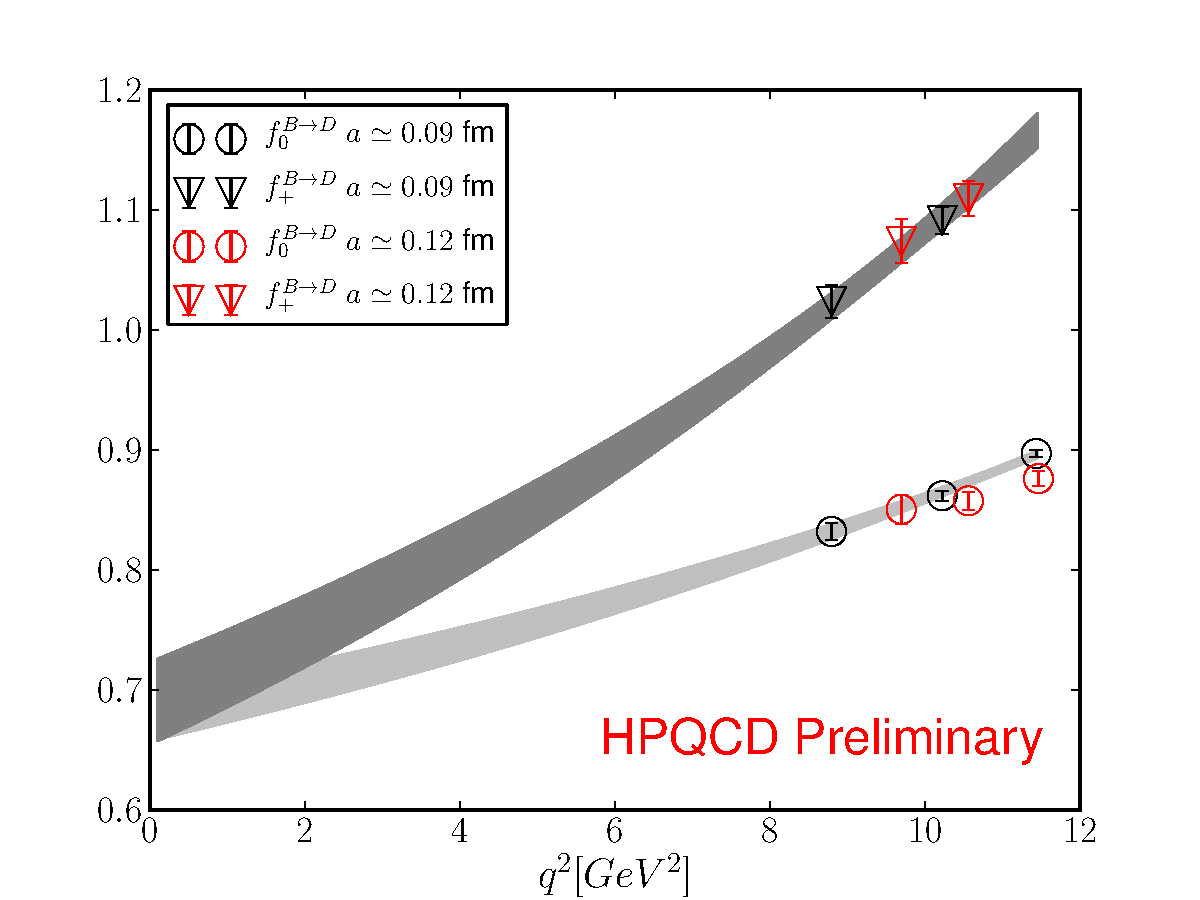
\includegraphics[width=1.0\linewidth]{images/BD_proceedings17.pdf}
  \label{fig:BD_ff}
\end{subfigure}%
\begin{subfigure}{.5\textwidth}
  \centering
  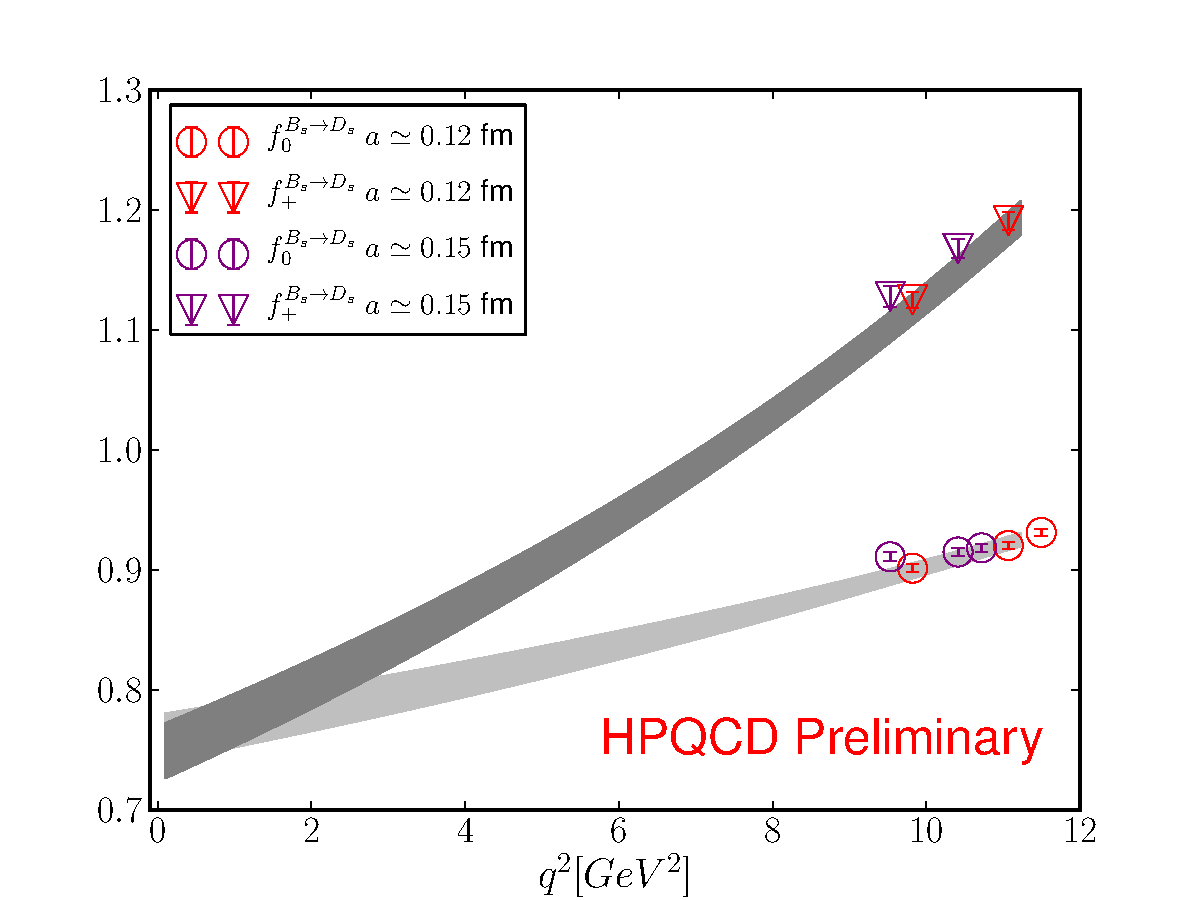
\includegraphics[width=1.0\linewidth]{images/BsDs_proceedings17.pdf}
  \label{fig:BsDs_ff}
\end{subfigure}
\caption{Form factors for the $B\to D$ (left) and $B_s \to D_s$ (right) cases. Errors on data points are statistical. The bands are produced from a fit to the data using \eqref{eq:zexpansion} as the fit form. \label{fig:ff}}
\end{figure}

A useful check of how well the discretization errors can be controlled as we add larger $|a\vec{p}_{D_{(s)}}|$ is to compute the speed of light $c = (E_{D_s}(\vec{p}_{D_s})^2 - M_{D_s}^2) / \vec{p}_{D_s}^2$ using our data. We can show that $c^2$ tends to unity in the continuum limit ($am_c,\left\vert a\vec{p}_{D_s} \right\vert\to 0$), see fig. \ref{fig:speedoflight} (see also \cite{Donald:2012ga}). 

\begin{figure}
\centering
\begin{subfigure}{.5\textwidth}
  \centering
  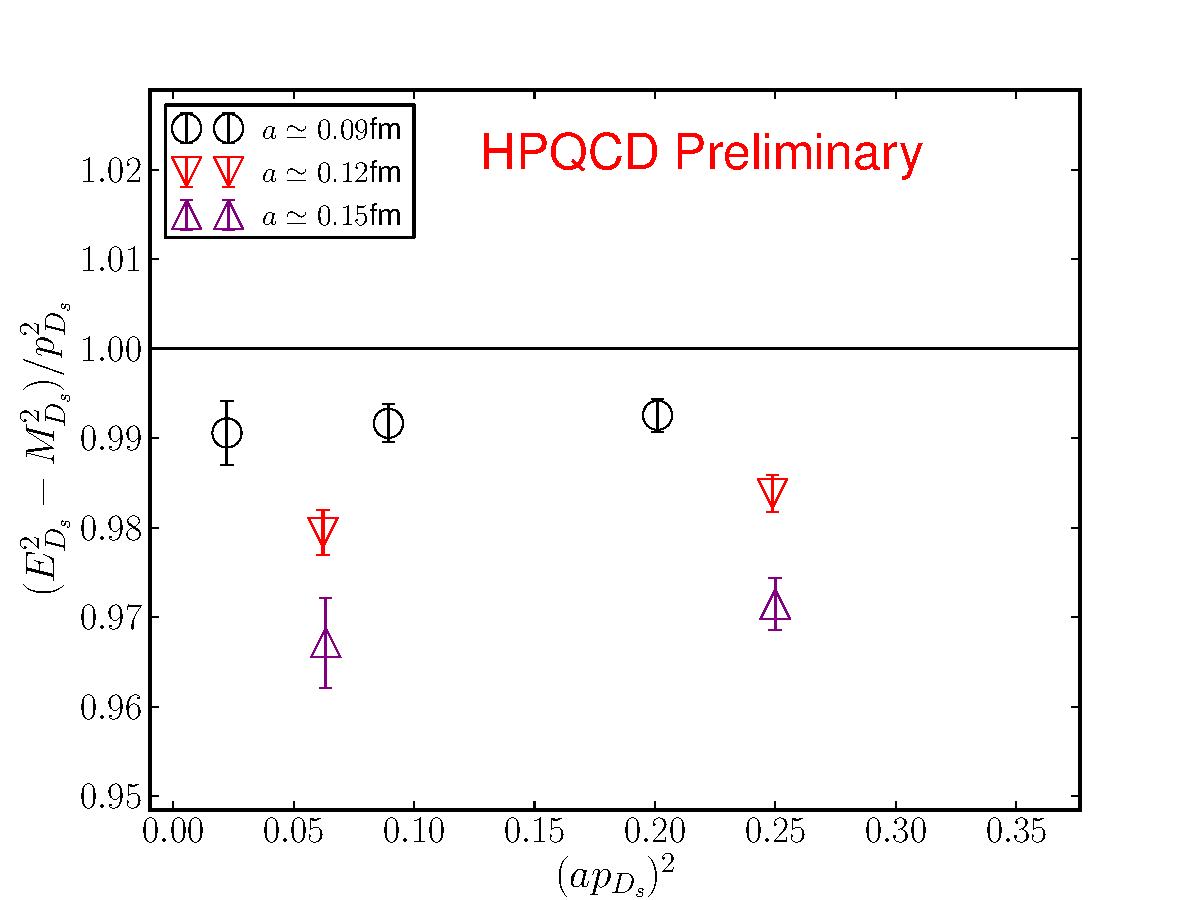
\includegraphics[width=1.0\linewidth]{images/c2_proceedings17.pdf}
  \label{fig:sub1}
\end{subfigure}%
\begin{subfigure}{.5\textwidth}
  \centering
  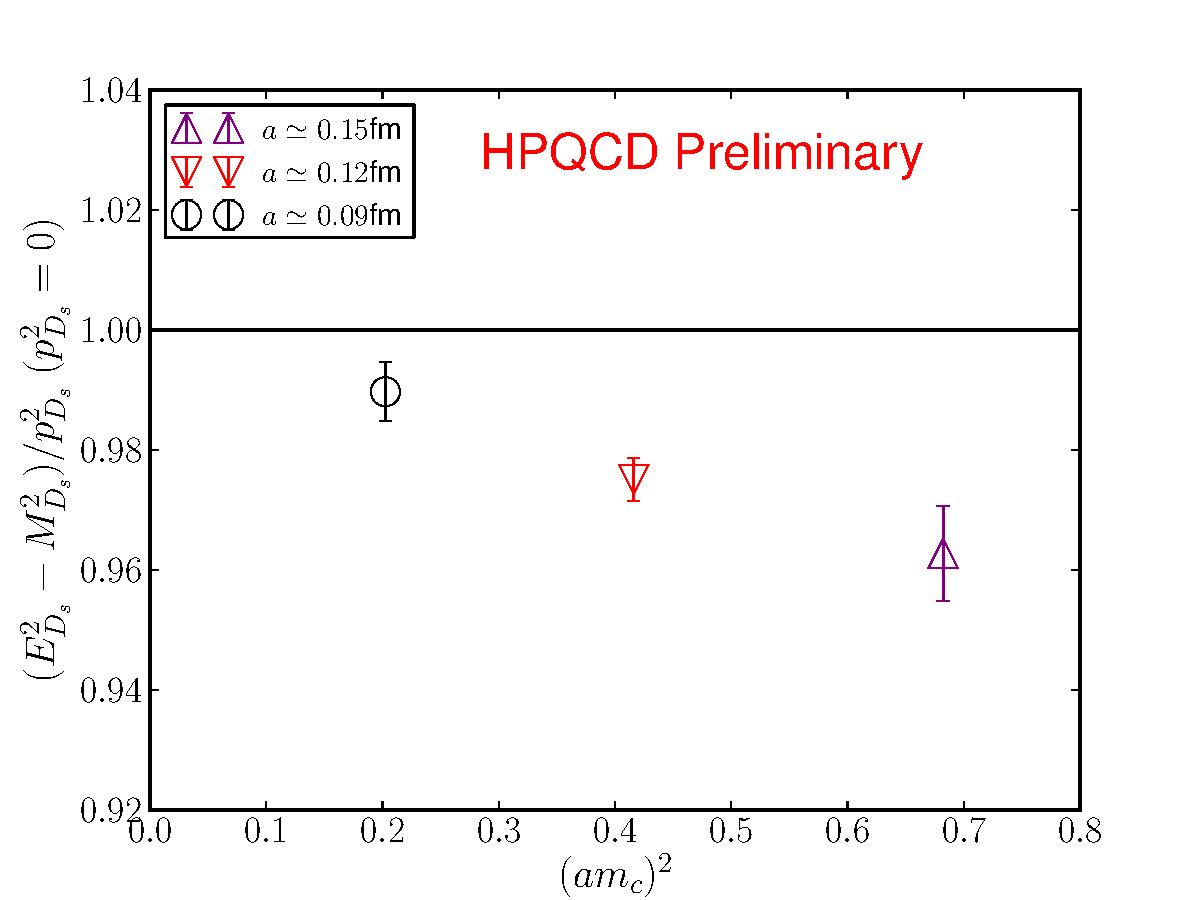
\includegraphics[width=1.0\linewidth]{images/c2p0_proceedings17.pdf}
  \label{fig:sub2}
\end{subfigure}
\caption{Left: The speed of light against $D_s$ momentum. Discretization errors cause this to differ from unity. Right: On each ensemble, the speed of light at $\left\vert a\vec{p}_{D_s} \right\vert=0$ is extrapolated from the $a\vec{p}_{D_s}\neq 0$ data (below $\left(a\vec{p}_{D_s}\right)^2 =0.5$), and plotted here. As can be seen, in the limit $am_c\to 0$, the speed of light tends towards unity, showing that discretization effects are controllable below $\left(a\vec{p}_{D_s}\right)^2 = 0.5$.}
\label{fig:speedoflight}
\end{figure}


\bibliographystyle{plain}
\bibliography{thesis}

\appendix


\section{Chiral Currents and Ward Identities}
\label{sec:ward}

The currents $V_{\mu}$ and $A_{\mu}$ are conserved in the Chiral limit (quark masses $\rightarrow 0$). This can be shown via Noether's theorem: consider a theory containing a number of fields $\{\varphi_i\}$, which transform under a group $G$ by
\begin{align}
	\varphi_i \rightarrow \varphi_i (x) - i\epsilon_a (x) F_{i,a}[\{\varphi\}]
\end{align}
It can be shown that there exists currents
\begin{align}
	J_a^{\mu} = -i{\partial \mathscr{L} \over \partial\partial_{\mu} \varphi_i} F_{i,a}
\end{align}
which obey
\begin{align}
	\label{eq:conservedJ1}
	J^{\mu}_a = {\partial \delta \mathscr{L} \over \partial \partial_{\mu} \epsilon_a } \\
	\partial_{\mu} J^{\mu}_a = {\partial \delta \mathscr{L} \over \delta \epsilon_a}	
	\label{eq:conservedJ2}
\end{align}
where $\delta\mathscr{L}$ is the result of an infinitesimal $G$ operation, i.e. $G$ : $\mathscr{L} \rightarrow \mathscr{L} + \delta\mathscr{L}$. From \eqref{eq:conservedJ2}, we see that if the theory is symmetric under the generator parameterised by $\epsilon_a$, then $J_a^{\mu}$ is a conserved current.
\\ \\
In the chiral limit, QCD with $N$ flavors has the accidental global symmetry ("chiral symmetry") $U(N)_L\times U(N)_R$:
\begin{align}
	q_{L/R} \rightarrow \text{exp}(-i\theta_a^{L/R} \lambda_a) q_{L/R}
	\label{eq:LRtransform}
\end{align} 
where $q$ is a vector in flavor space, and $\lambda_a$ are the generators of $U(N)$ in the fundemental representation and acts on flavor. Applying \eqref{eq:conservedJ1} and \eqref{eq:conservedJ2} to QCD we get the conserved currents:
\begin{align}
	J_{L/R}^{\mu,a} &= \bar{q}_{L/R} \gamma^{\mu} \lambda_a q_{L/R} \\
	\partial_{\mu} J_{L/R}^{\mu,a} &= 0
\end{align}
$J_{L/R}$ are often expressed instead in terms of {\it{vector}} and {\it{axial}} currents
\begin{align}
	V^{\mu,a} &= J^{\mu,a}_L + J^{\mu,a}_R = \bar{q} \gamma^{\mu} \lambda_a q \\
	A^{\mu,a} &= J^{\mu,a}_L - J^{\mu,a}_R = \bar{q} \gamma^{\mu} \gamma_5 \lambda_a q
\end{align}
which are conserved currents corresponding to the vector and axial symmetries $U(N)_V$ and $U(N)_A$, consisting of simultanious $L/R$ transformations above with constraints $\theta_a^{L} = \pm \theta_a^{R}$. Vector and axial currents between any two individal flavours, i.e.
\begin{align}
	\label{eq:individualflavs1}
	V^{\mu}_{ij} = \bar{q_i} \gamma^{\mu} q_j \\
	A^{\mu}_{ij} = \bar{q_i} \gamma^{\mu} \gamma_5 q_j
	\label{eq:individualflavs2}
\end{align}
are also conserved, since they can be constructed from linear combinations of $V^{\mu,a}$ and $A^{\mu,a}$.
\\ \\
$U(N)$ can be broken up into $SU(N)\times U(1)$, where $U(1)$ is a singlet transformation, i.e., of the form of \eqref{eq:LRtransform} with $\lambda = 1$. When QCD is quantized, it develops an anomaly which breaks the singlet axial symmetry. This reduces the symmetry group to $SU(N)_V\times SU(N)_A\times U(1)_V$, and prevents the corresponding axial singlet current $A^{\mu,0}$ from being conserved.
\\ \\
In the case of non-zero quark mass, the chiral symmetry is broken. This leads to \eqref{eq:conservedJ2} for the vector and axial currents evaluating instead as
\begin{align}
	\partial_{\mu} V^{\mu,a} &= i\bar{q} [ M,  \lambda_a ] q \\
	\partial_{\mu} A^{\mu,a} &= i\bar{q} \{ M, \lambda_a \} q 
\end{align}
where $M$ is the quark mass matrix in flavor space. These are the parially conserved axial and vector current identities (PCAC and PCVC). By taking a linear combination of these equations, one can derive PCAC and PCVC for individual flavors:
\begin{align}
	\partial_{\mu} V_{ij}^{\mu} &= i(m_i - m_j) \bar{q_i} q_j \equiv i(m_i - m_j) S_{ab} \\
	\partial_{\mu} A_{ij}^{\mu} &= i(m_i - m_j) \bar{q_i} \gamma_t q_j \equiv i(m_i - m_j) P_{ij}
\end{align}
We refer to $S$ as the scalar current and $P$ as the pseudoscalar. These identities translates straightforwardly to expectation values:
\begin{align}
	\label{eq:PCVC}
	(p_1 - p_2)_{\mu} \langle \psi(p_2) | V^{\mu}_{ij} | \phi(p_1) \rangle &= (m_i - m_j) \langle \psi(p_2) | S_{ij} | \phi(p_1) \rangle \\
	(p_1 - p_2)_{\mu} \langle \psi(p_2) | A^{\mu}_{ij} | \phi(p_1) \rangle &= (m_i - m_j) \langle \psi(p_2) | P_{ij} | \phi(p_1) \rangle
\end{align}
where $| \psi(p) \rangle$ and $| \phi(p) \rangle$ are arbitrary states containing momentum $p$.
\\ \\
These are powerful tools for connecting expectation values of different currents. For example, by combining \eqref{eq:PCVC} and \eqref{eq:formfactors}, we see that:
\begin{align}
	\langle P_2(p_2) | S_{ij} | P_1(p_1) \rangle = {M_1^2 - M_2^2 \over m_i - m_j} f_0(q^2)
\end{align}
Hence we have an extra route to accessing $f_0$. In a lattice simulation which computes expectation values of $V^{\mu}$, one could constrain $f_0$ by also computing the scalar current on the lattice, then use the rest of the information in $V^{\mu}$ to constrain $f_+$.

\section{The Doubling Problem}
\label{sec:doublingprob}

The interacting Dirac action is most naively discretised with
\begin{align}
 S_F &= \sum_{x,\mu} \bar{\psi}(x) \gamma_{\mu} \nabla_{\mu} \psi(x) + m\sum_x \bar{\psi}(x) \psi(x),
 \label{eq:naivefermions}
\end{align}
where $\nabla_{\mu}$ is the gauge covariant finite difference operator,
\begin{align}	
	\nabla_{\mu} \psi(x) = {1\over 2a} ( U_{\mu} (x) \psi(x+a\hat{\mu}) - U^{\dagger}_{\mu}(x-a\hat{\mu})\psi(x-a\hat{\mu}) ).
\label{eq:lat_derivative}
\end{align}
An issue arises with fermions on the lattice, known as the doubling problem. $S_F$ is invariant under a so-called "doubling symmetry", which is generated by
\begin{align}
	\label{eq:doublingsymmetry}
	\psi(x) & \to \mathcal{B}_{\mu} \psi(x) \equiv  (-1)^{x_{\mu}/a} \gamma_{5\mu} \psi(x) \\
	\bar{\psi}(x) & \to \bar{\psi(x)}\mathcal{B}^{\dagger}_{\mu} \equiv (-1)^{x_{\mu}/a} \bar{\psi}(x) \gamma^{\dagger}_{5\mu}
\end{align}
where $\gamma_{5\mu} = i\gamma_{\mu}\gamma_5$. The product space of these form a group of 16 elements $\{\mathcal{B}_{\zeta}\}$, labeled  by vectors $\zeta$ with $\zeta_{\mu}\in \mathbb{Z}_2$ (e.g.the element $\mathcal{B}_{0}\mathcal{B}_{1}$ is labeled by $\zeta=(1,1,0,0)$).
\\ \\
The physical signifiance of this symmetry can be seen when we study it's effect on the action. First, notice that
\begin{align}
	\mathcal{B}_{\mu} \psi(x) & = \gamma_{5\mu} \sum_k \tilde{\psi}(k) e^{i(k+{\pi\over a}\hat{\mu})\cdot x} \\
	& = \gamma_{5\mu} \sum_k \tilde{\psi}(k-{\pi\over a}\hat{\mu})e^{ik\cdot x}
\end{align}
where $k$ is a set of discrete 4-momenta. The action in momentum space can be written as
\begin{align}
	S = \sum_k \bar{\tilde{\psi}}(k) M(k) \tilde{\psi}(k)
\end{align}
after the operation of $\mathcal{B}_{\mu}$ it becomes
\begin{align}
	S \to \sum_k \bar{\tilde{\psi}}(x)(k) \gamma_{5\mu} M(k+{\pi\over a}\hat{\mu})\gamma_{5\mu} \tilde{\psi}(k)
\end{align}
Since we know $S$ is invariant under this transformation, it must be true that $\gamma_{5\mu} M(k+{\pi\over a}\hat{\mu})\gamma_{5\mu} = M(k)$, and therefore
\begin{align}
	M^{-1}(k+{\pi\over a}\hat{\mu}) = \gamma_{5\mu} M^{-1}(k) \gamma_{5\mu}
	\label{eq:doubling}
\end{align}
$M^{-1}$ is the propagator for the fermion field, so \ref{eq:doubling} shows that the spectrum of the fermion is periodic, with a period of $\pi/a$. We expect a pole in $M^{-1}(k)$ where $k \sim m$, where $m$ is the pole mass of the fermion, but there will now be a second pole at $m + \pi/a$. This will be around the natural cutoff imposed by the lattice $1/a$, and any higher poles like $m+2\pi/a$ is far above the cutoff so will not contribute.  
\\ \\
Generalizing this argument to all elements of the doubling symmetry, we see that
\begin{align}
	M^{-1}(k+{\pi\over a}\zeta) = \gamma_{5\mu} M^{-1}(k) \gamma_{5\mu}
\end{align}
leading to 16 poles in the fermion specturm, therefore 16 distinct excitations (called \textit{tastes}).
\\ \\
We now show that there are only 4 tastes in the staggered quark formalism. 
One can isolate a single taste by a block-scaling procedure:
\begin{align}
	\psi^{(\zeta)}(x_B) = \sum_{\delta x_{\mu} \in \mathbb{Z}_2} \mathcal{B}_{\zeta} \psi(x_B + \delta x)
\end{align}
For example, for $\zeta = 0$, it would only contain the original non-doubler taste, since all other poles at $|k|\sim\psi/a$ have been integrated out. For $\zeta \neq 0$, the $\mathcal{B}_{\zeta}$ operator pushes the $\zeta$ doubler to where the $\zeta=0$ taste originally was in $k$ space, then the blocking procedure integrates out the rest. Now writing this isolated taste in terms of $\chi$ we arrive at:
\begin{align}
	\psi^{(\zeta)}(x_B) = \sum_{\delta x_{\mu} \in \mathbb{Z}_2} \Omega(\delta x) \mathcal{B}_{\zeta}(0) \chi(x+\delta x)
\end{align} 
Recall we set $\chi(x) = (\chi_1(x),0,0,0)$. The product $\Omega(\delta x) \mathcal{B}_{\zeta}(0)$ is simply a product of gamma matrices, so can only serve to "scramble" the elements of $\chi$. Then, in the staggered formalism, all 16 tastes $\psi^{(\zeta)}$ amount to only 4 distinguishable fermions: $(\chi_1,0,0,0)$, $(0,\chi_1,0,0)$, $(0,0,\chi_1,0)$, $(0,0,0,\chi_1)$ (with factors of (-1) and $i$).


\section{Signal/Noise Ratio}
\label{sec:signalnoise}

One of the main obstacles in our calculation is the \textit{signal degredation} of correlation functions computed on the lattice.
\\ \\
A random variable $x$ has mean and standard deviation
\begin{align}
	&\hat{x} = \langle x \rangle \\
	&\sigma^2 = {1\over N} ( \langle x^2 \rangle - \langle x \rangle^2 ),
\end{align}
where $N$ is the size of the sample. So the (square of) the signal/noise ratio is
\begin{align}
	{\hat{x}^2\over \sigma^2} = N \left( {\langle x^2 \rangle \over \langle x \rangle^2} - 1 \right) ^{-1}.
\end{align}
Consider 2 point correlators where $x = \Phi^{\dagger}(t) \Phi(0)$, where $\Phi$ is a meson operator with zero spacial momentum.
\\ \\
$\langle x^2 \rangle$ and $\langle x \rangle$ can be written as
\begin{align}
	\langle x \rangle &= \sum_k {1\over 2E_n} \langle 0 | \Phi^{\dagger}(t) | \lambda_n \rangle \langle \lambda_n | \Phi(0) | 0 \rangle e^{-E_n t} \simeq_{t\to\infty} e^{-E_0 t}\\
	\langle x^2 \rangle &= \sum_n {1\over 2E_n} \langle 0 | \Phi^{\dagger 2}(t) | \lambda_n \rangle \langle \lambda_n | \Phi^2(0) | 0 \rangle e^{-E_n t} \simeq_{t\to\infty} e^{-E'_0 t}
\end{align}
where we have assumed the ratio of matrix elements and energies are $\mathcal{O}(1)$. The two ground state energies $E_0$ and $E'_0$ need not be the same, since the lowest states for which 
$\langle \lambda_n | \Phi(0) | 0 \rangle \neq 0$ and $\langle \lambda_n | \Phi^2(0) | 0 \rangle \neq 0$ may differ. 
\\ \\
The operator $\Phi^2$ will contain two quark and two antiquark operators, connected by some matrices in spin space. $\Phi^2$ can create a combination of all possible 2 meson states where the mesons are made of the available quark species, and quantum numbers. For example, If $\Phi$ is a pion, $\Phi^2$ is a 2 pion state, and $E_0' = 2m_{\pi}$. If $\Phi$ is a $D_s$ meson, then $E_0' = m_{\tilde{\pi}} + m_{\eta_c}$ ($\tilde{\pi}$ is a pseudoscalar $s\bar{s}$ state).
\\ \\
Define $\mu_0 = E_0'/2$. Then
\begin{align}
	{\hat{x}^2\over \sigma^2} \simeq N \left( e^{-2(\mu_0 - m_{\Phi})t} - 1 \right) ^{-1}
\end{align}
In the case of pions, $\mu_0 = m_{\Phi}$, the ratio becomes simply $\sim N$. For mesons heavier than the pion, $\mu_0 < m_{\Phi}$, so at large times $e^{-2(\mu_0 - m_{\Phi})t} >> 1$, and upon taylor expanding the inverse of this phase we arrive at
\begin{align}
	{\hat{x}\over\sigma} \simeq \sqrt{N} e^{-(m_{\varphi} - \mu_0)t}
	\label{eq:signaltonoise}
\end{align}
From this we see there are 3 variables which effect the quality of the signal:
\begin{enumerate}
\item
The size of the sample $N$.
\item
At large $t$, the correlators undergo {\it{signal degredation}}, i..e, become dominated by noise.
\item
The degree of signal degradation is decided by $m_{\varphi} - \mu_0$. Heavier mesons will tend to experience more signal degredation.
\end{enumerate}
Relevant to our calculation is how giving mesons non-zero spacial momenta $\underline{p}$ can exaserbate this problem. In this case, $m_{\Phi}$ in \eqref{eq:signaltonoise} is replaced with $\sqrt{m_{\Phi}^2+\underline{p}^2}$. As $\underline{p}$ increases, the signal/noise ratio will degrade more and more and statistics will suffer.
\\ \\
In the $B_s\to D_s l\nu$ calculation, to deduce form factors over the whole range of $q^2$ values, we need to simulate the process with the $D_s$ having a range of momenta $0 < |\underline{p}| < 2.32$GeV, as discussed in sec. \ref{sec:formfactors}. Correlation functions at the higher end of this range may be too noisy for any meanigful results to be extracted. We are investigating ways of taming this problem, see sec. \ref{sec:highmomenta}.